\documentclass[12pt,a4paper]{report}

\usepackage{dolgozat}

\usepackage{hyperref}

\usepackage{listings}
\usepackage{python}
\usepackage{cpp}

\linespread{1.2}

\begin{document}

\pagestyle{empty} %a címlapon ne legyen semmi=empty, azaz nincs fejléc és lábléc

\begin{flushleft}
\textsc{\bfseries Miskolci Egyetem}\\
Gépészmérnöki és Informatikai Kar\\
Általános Informatikai Intézeti Tanszék
\end{flushleft}

%A fõiskola logoja
{\large
\begin{center}
\vglue 1truecm
\textbf{\huge\textsc{Szakdolgozat}}\\
\vglue 1truecm

\epsfig{file=cimlap/ME_logo.eps, width=4.8truecm, height=4truecm}\\
\textbf{\textsc{Miskolci Egyetem}}
\end{center}}

\vglue 1.5truecm %függõleges helykihagyás

%A szakdolgozat címe, akár több sorban is
{\LARGE
\begin{center}
\textbf{Éttermi rendelésnyilvántartó rendszer}
\end{center}}

\vspace*{2.5truecm}
%A hallgató neve, évfolyam, szak(ok), a konzulens(ek) neve
{\large
\begin{center}
\begin{tabular}{c}
\textbf{Készítette:}\\
Gábori Péter Márk\\
Mérnökinformatikus BSc
\end{tabular}
\end{center}
\begin{center}
\begin{tabular}{c}
\textbf{Témavezetõ:}\\
Piller Imre, egyetemi tanársegéd
\end{tabular}
\end{center}}
\vfill
%Keltezés: Hely és év
{\large
\begin{center}
\textbf{\textsc{Miskolc, 2017}}
\end{center}}

\newpage


\cleardoublepage
\pagenumbering{gobble}
\tableofcontents
\cleardoublepage
\pagenumbering{arabic}

\newpage

\pagestyle{fancy}

\chapter{Bevezetés}

A világ felgyorsult, az emberek állandó rohanásban vannak, nem mindig jut idő olyan alapvető dolgok elvégzésére, mint például a főzés. Az éttermek látogatása is egy idő igényes tevékenység, ezért megnőtt a kereslet az ételek házhoz rendelésére. Az interneten számos alternatívát találhatunk ételrendelős webes alkalmazások terén, de ezek nem működnek megfelelően, nem egyértelmű a használatuk és nem felhasználóbarát alkalmazások kialakítása. A dolgozatom célja egy olyan webalkalmazás készítése, amely több étterem adatbázisát kezeli, ezáltal megkönnyíti az ételrendelést a felhasználók számára, mivel egy weboldalon megtalálhatják számos étterem kínáltatát, és kiválaszthatják a számukra legszimpatikusabbat. A dolgozatomban összpontosítani fogok egy letisztult, egyértelmű, könnyen kezelhető felhasználói felület kialakítására különböző szűrési lehetőségekkel. Továbbá az üzletvezetők feladatának, az éttermek menedzselésének megkönnyítésére online étterem kezelő felülettel, statisztikákkal, kimutatásokkal, melyek elengedhetetlenek egy sikeres vállalkozáshoz.

Az alkalmazásom szerver oldalon Python/Flask keretrendszert, míg kliens oldalon AngularJS-t fog használni. Az adatokat relációs adatbázis tárolja majd, amelyhez a keretrendszer SQLAlchemy ORM-en keresztül fog csatlakozni.

A dolgozatom első részében, el fogom helyezni az alkalmazásomat a piacon, bemutatom az étterem és a rendelésnyilvántartás módjait, és néhány konkurens programot. Azután szeretném bemutatni a használni kívánt technológiákat, és ismertetem az alkalmazásom felépítését, főbb részeit. Ezt követően részletezem az SQL adatbázisom felépítést, majd leírom az alkalmazás kliens és szerveroldali megvalósítását. És végül kitérek az elkészített alkalmazásom tesztelésének lehetőségeire is.
\chapter{Éttermi nyilvántartás}

Itt ki kell majd fejteni, hogy melyek azok a dolgok, amiket egy étteremnek nyilván kell tartania. Ebben a részben még nem kell belemenni a technikai részletekbe, hanem azt kell körüljárni, hogy mi a konkrét problémakör, annak mely részeire fog koncentrálni a dolgozat további része.

Elterjedt megoldások:

* Ebben a részben össze kell szedni, hogy milyen elérhető megoldások vannak az éttermek számára.
* Itt érdemes minél több elérhető megoldást összeszedni, és ha lehet diagramokat, összehasonlító táblázatokat is készíteni hozzá.
* A bemutatott megoldásokat majd mindenképpen be is kell hivatkozni.

% TODO: Összeszedni táblázatba a funkciókat.

Pl.:

program neve | felhasználókezelés | profil | könyvelés | feladatkezelés | készletnyilvántartás |

profil: általános webshop ... teljesen egyedi, éttermekre szabott.
feladatkezelés: pénztárgép szoftver is-e egyben? Mennyire

Kb. 10 leginkább elterjedt program.

% \section{Éttermi nyilvántartás}

Az éttermi nyilvántartás egy roppantul összetett problémakör. Az ilyen szoftverek tervezésénél figyelembe kell venni, hogy nincs két egyforma vendéglátó egység, tehát a szoftvert mindig az adott vállalkozáshoz kell igazítani. Nyilván kell tartani a rendeléseket, a raktárkészletet, a felhasználókat, törzsvendégek kezelését. A szoftverrel szemben elvárás, hogy megkönnyítse a szoftverrel dolgozók munkáját, átláthatóvá tegye az üzletvezetők számára az üzlet menetét és az ellenőrzést. Szintén elvárás, hogy könnyen kezelhető és rugalmasan bővíthető legyen.

\subsection{Rendelésnyilvántartás}

Rendelések esetén számos adatot nyilván kell tartani. Fontos, hogy ki rendelt, mikor, melyik étteremből, mit, mennyit és mivel fizetett. Menedzselni kell futárszolgálatot, betartani a kiszállítási időt. Biztosítani kell a vásárlók számára pontos leírást az ételekről, választási lehetőséget a fizetési lehetőségek között, estleg vegyes fizetési lehetőségeket egy számlán belül.

\subsection{Készletnyilvántartás}

Vannak éttermi nyilvántartó szoftverek, melyek lehetőséget biztosítanak teljes körű raktárkészlet kezelésre, egy vagy akár több raktárral is. Ebbe beletartozik az alapanyagok bevételezése, selejtezés, abban az esetben, ha több raktár is van, akkor raktárok közötti átvételezés.
Ebbe a problémakörbe tartozhat még a menü összeállítása, előrendelések kezelése, a termékekhez tartozó receptúrák kezelése, tehát nyilvántartása és módosítása.

\subsection{Törzsvendégek kezelése}

A vásárlók teljeskörű nyilvántartása az ilyen típusú szoftverek esetén alap elvárás. A rendszeresen vásárló felhasználók számára nyújtani kell valamilyen fajta plusz szolgáltatást, amivel meg lehet hálálni a hűségüket, és el lehet azt érni, hogy továbbra is ezt a szoftvert használják. Erre a problémára nyújtanak megoldást a különböző törzsvásárlói kedvezmények.

\subsection{Ellenőrzés}

Egy sikeres vállalkozáshoz szükség van a folyamatos ellenőrzésre, az üzletvezetőnek mindig át kell látnia az üzlet menetét. Az ilyen típusú nyilvántartó rendszerek egy része lehetőséget biztosít a termékek szerinti fogyások kimutatására, ez egy nagyon fontos statisztika, amely megmutatja, hogy egy adott időszakban melyik termék volt a legnépszerűbb, tehát fogyott belőle a legtöbb, illetve, hogy melyikből fogyott a legkevesebb. Biztosítják az alapanyagok készletszintjének figyelését.

Fontos statisztikákat, grafikonokat állítanak elő egy adott időszakra, melyek nélkülözhetetlenek a további üzleti lépések meghozatalához, a sikeres üzleti élethez. Kimutatások a pillanatnyi alapanyag készletről, ezeknek lekérdezése, a lekérdezések és kimutatások exportálása.

\subsection{Elterjedt megoldások}

Az internetet böngészve számos étterem nyilvántartó szoftvert lehet találni. Vannak köztük online webalkalmazások, és letölthető desktop alkalmazások is. Összeszedtem a már létező alternatívák közül a Magyarországon legelterjedtebbeket, és egy táblázatban néhány szempont alapján összehasonlítottam őket (\ref{tab:features}. táblázat).

\begin{table}
\centering
\begin{tabular}{|l|c|c|c|c|c|}
\hline
Program neve & felhasználókezelés & profil & könyvelés & feladatkezelés & készletnyilvántartás \\
\hline
eSystem & van & általános webshop & van & igen & igen \\
\hline
R-keeper & nincs & teljesen egyedi & nincs & igen & igen \\
\hline
MultiStore & nincs & teljesen egyedi & van & igen & igen \\
\hline
Stand-Mágus & van & teljesen egyedi & van & igen & igen \\
\hline
\end{tabular}
\caption{Elterjedt funkciók}
\label{tab:features}
\end{table}

A táblázat első oszlopában a szoftver neve szerepel. A második oszlopban a felhasználókezelés, ami azt takarja, hogy a szoftver funkció között van e vendég nyilvántartás, tehát, hogy lehet e regisztrálni a vendégeket. A harmadik oszlopban a szoftver profilját, arculatát jellemeztem. A negyedik oszlopban azt vizsgáltam, hogy van e integrált könyvelés funkció az alkalmazásban. Az 5. oszlopban feladatkezelés alatt azt értettem, hogy a pénztárgép funkcióit is a szoftver látja e el. A hatodik azaz utolsó oszlopban a szoftver raktár készlet kezelését vizsgáltam.

Az én alkalmazásom a vásárlók teljes körű nyilvántartására, rendelések nyilvántartására és az ezekből alkotott kimutatásokra, statisztikákra fog összpontosulni. Az alkalmazásom célja, a házhoz szállítást nyújtó éttermek összegyűjtése, az üzletvezetők feladatának, éttermek menedzselésének megkönnyítése, és a rendelők számára a minél egyszerűbb ételrendelés biztosítása. Az hasonló célú és felépítésű szoftvereket online ételrendelési portálnak szokták nevezni.

A magyar piacon jelenleg három online ételrendelési portál óriás van, a NetPincér, a Pizza.hu és a Falatozz.hu. Ezek a portálok közvetítő szerepet játszanak a megrendelő és a kiszállítást lebonyolító étterem között. Az éttermeknek ez egy nagyon jó marketing fogás, segít nekik az ügyfélkör kibővítésében, a megrendelőknek, meg leegyszerűsítik az online ételrendelést, azzal, hogy egy oldalon megtalálják a környéken lévő összes vendéglátó egység kínálatát.

Az alkalmazásom abban különbözik ezektől az online étrendelési portáloktól, hogy míg ezek a portálok úgymond csak közvetítő szerepet vállalnak, nem feltétlenül tartják nyilván az adatokat, a partner cégek egyébként is rendelkeznek egy saját étterem nyilvántartói rendszerrel és általában webes rendelő felülettel is. Addig az általam készített alkalmazás biztosítja a rendelésnyilvántartást, a vásárlónyilvántartást és a szerzett adatokból olyan statisztikákat, kimutatásokat állít elő, melyek elengedhetetlenek egy sikeres vállalkozáshoz.

Ez nem feltétlen jó így fejezet címnek, pontosabban ezen a témán belül több fejezet is lehet, attól függően, hogy majd mivel és hogy sikerül elkészülni.

Itt kb. olyasmire kell gondolni, mint
- rendelések nyilvántartása,
- promóciók, törzsvásárlói kedvezmények megvalósítása a rendszerben,
- nyersanyagok nyilvántartása,
- rendelési statisztikák, elemzés, megjelenítés,
- ...

Annyi biztos, hogy a címnek megfelelően a rendeléseket majd nyilván kell tartani. A többi ahhoz kapcsolható funkció, de csak akkor célszerű vele foglalkozni, ha az alapfunkciók már megvannak.

A tervezéséről szóló dolgokat az alkalmazás felépítésénél is el lehet kezdeni, de ott még inkább csak az interfészekre, az API jellegére, konvenciókra, illesztési módokra vonatkozóan.

Magában az implementációba annyira kell csak majd belemenni az alapfunkciók bemutatásánál, hogy a kiemelt kódpéldák alapján át lehessen tekinteni a rendszer egészét, és a leírás alapján aki akarja hellyel-közzel tuda is reprodukálni a rendszert.

\section{Az alkalmazás alapfunkciói}

Az alkalmazásom lényegében éttermek és rendelések adatainak nyilvántartására fog szolgálni. Ebben a fejezetben az alap funkcionalitásokat fogom tárgyalni.

\section{Bejelentkezés/ regisztráció}

Az alkalmazásom egyik alap funkcionalitása a felhasználókezelés lesz. Csak regisztrált felhasználók számára lesznek elérhetőek a szolgáltatások, a kezdőlapon lesz lehetőség a bejelentkezésre, vagy regisztrációra. Alapvetően két felhasználói csoportot lehet majd megkülönböztetni, a vásárlókat és az étterem tulajdonosokat. A két csoport eltérő jogosultsági körrel fog rendelkezni, és más-más szolgáltatások lesznek számukra elérhetőek.

\section{Vásárlók funkciói}

\subsection{Böngészés az éttermek között}

A vásárlóknak lehetőségük lesz az adatbázisban szereplő éttermek kínálatai között böngészni. Szűrési feltételek megadásával szűkíthetik a kilistázott éttermek listáját, hogy megtalálják a számukra legszimpatikusabbat.
A kívánt étterem kiválasztása után a server kilistázza az adott étterem által kínált termékeket. A termékek között is lesz lehetőség szűrésre például típus szerint. A megrendelendő termékeket a vásárló belehelyezheti a kosárba. A kosár tartalma egy angular változóban lesz letárolva. A kosár tartalma is módosítható lesz.

\subsection{Rendelés}

A rendelés véglegesítése előtt a vásárlónak lehetősége lesz kiválasztani a kívánt fizetési módot. Rendelés során a kosár tartalma elküldésre kerül a servernek. A server létrehozza a szükséges order és \texttt{order\_meals} objektumokat, majd letárolja őket az adatbázisban. A rendelésről visszajelzést fog kapni a vásárló és az étterem tulajdonosa is. A rendelések adatait később statisztikák, kimutatások készítésénél lehet majd felhasználni.

\subsection{Felhasználói adatok}

A felhasználók számára lesz egy szolgáltatás, amely kilistázza az adott account adatait.

\subsection{Jelszó módosítás}

A felhasználói adatok kilistázása mellett lehetőség lesz a jelszó módosításra is. Ehhez egy űrlap kitöltésére lesz szükség, ahol meg kell majd adni az aktuális érvényben lévő jelszó mellett az új jelszót is. Az megadott adatokat server oldalon fogom vizsgálni, ha megadott jelszó megegyezik a felhasználói fiók tényleges jelszavával, akkor a server elvégzi a szükséges adatbázis módosításokat.

\subsection{Törzsvásárlói kedvezmények}

A vásárlók hűségének honorálása miatt, minden leadott rendelés után jutalompontokat írunk jóvá a rendelést leadó felhasználó javára. A pontokat fizetéskor lehet majd beváltani, ilyenkor a pontok összege levonásra fog kerülni a rendelés összegéből.

\section{Étterem tulajdonosi funkciók}

Az étterem tulajdonosoknak nyújtott szolgáltatások az éttermeik menedzselése, új éttermek felvitele a rendszerbe, és az éttermeikkel kapcsolatos statisztikák kimutatása.

\subsection{Éttermeim}

Az étterem tulajdonos számára adott lesz egy funkció, melynek segítségével ki tudják majd listázni a tulajdonukban lévő éttermeket. A felhasználó minden éttermének megtudja majd nézni az termék kínáltát, az étterembe leadott rendeléseket és tudja majd módosítani az adott étterem adatait.

\subsection{Termékek módosítása}

A felhasználó minden egyes éttermének meg tudja nézni a termékkínálatát. A termékekre lesz szűrési lehetőség a köztük történő navigáció megkönnyítése érdekében. Az egyes termékeket lehet majd törölni és módosítani, illetve lesz lehetőség újabb termékek felvitelére az adatbázisba.
A termékek módosítása egy űrlap kitöltésével fog kezdődni, ahol meg kell majd adni a módosítandó adatokat. Ezeket az adatokat a server fogja megkapni, feldolgozni, és végrehajtani az adatbázisban.

\subsection{Termékek törlése}

A törlendő termékre a felhasználó meghívhatja a termék törlése funkciót, ekkor a termék letárolódik egy angular változóba és elküldésre kerül a servernek. A server feldolgozza a kapott adatokat, az adatbázisból törli a megfelelő azonosítójú terméket, majd véglegesíti az adatbázis módosításokat.

\subsection{Termék felvitel}

A termék felvitel funkció meghívásakor a felhasználó egy űrlapot fog látni. Miután kitöltötte a megfelelő mezőket, a felvitt adatok elküldésre kerülnek. A server a kapott adatokat feldolgozza, és létrehoz egy meal objektumot az adatok felhasználásával. Ezt az objektumot felviszi az adatbázisba, majd véglegesíti az adatbázis módosításokat.

\subsection{Étterem létrehozása}

A felhasználó éttermeket is hozzátud adni az adatbázishoz. Egy étterem felviteléhez mindössze egy űrlapot kell kitölteni a megfelelő adatokkal. Kitöltés után az adatokat az angular továbbítja a servernek. A server a kapott adatokból létrehoz egy új restaurant objektumot, és menti az adatbázisba.

\subsection{Étterem módosítsa}

Egy étterem módosításához egy űrlap kitöltésére lesz szüksége, amire a módosítandó adatokat kell felvinni. Az űrlap elküldése után az angular továbbítja az adatokat a servernek, ami feldolgozza és véglegesíti a módosításokat.

\subsection{Rendelések}

A felhasználó mindegyik éttermére megtudja majd hívni a rendelések funkciót, amely kilistázza az adott étteremben leadott rendeléseket.

\subsection{Statisztikák}

Az étterem tulajdonosok számára lesz egy szolgáltatás, amely statisztikákat, grafikonokat állít elő egy adott időszakra, melyek nélkülözhetetlenek a további üzleti lépések meghozatalához, a sikeres üzleti élethez. A felhasználók megnézhetik például hogy melyik ételtípusból rendelik a legtöbbet, a különböző fizetési módok gyakoriságát, vagy például a felhasználók rendelésszámának eloszlását.

\section{Statisztikai jellegű elemzések}

Felhasználói szokások elemzése

Rendelések száma (idő függvényében)
Rendelések összege
Fizetési módok gyakorisága
Ételek típusai
Felhasználók rendelésszámának eloszlása
Nap melyik szakában történt a rendelés (ehhez is eloszlás)

Felhasználók osztályozása/klaszterezése
- osztályozásnál eleve tudjuk, hogy mi a csoport jellemzője.
- klaszterezésnél adottak a mintáink, szeretnénk megtudni, hogy milyen csoportok vannak benne.

\section{Ajánlórendszer}

Piaci kosár elemzés

Amit meg kellene nézni:
- Milyen termékhez milyen másik terméket érdemes ajánlani?
- Mikor célszerű az akciókat meghírdetni és milyen termékekre vonatkozóan? (Például hónap elején-végén, karácsonykor, szezonalitást vizsgálni)
- Felhasználónként mikor lehet külön üzenetet küldeni egy-egy akcióról? (Észrevétel: Nem érdemes túl sok akciót küldeni gyakran, mert spam lesz belőle.)

\Chapter{Az alkalmazás felépítése}

\Section{Felhasznált eszközök és technológiák}

A feladatom webalkalmazás készítése éttermek és rendelések adatainak nyilvántartásához. Ennek megvalósításához a Python programozási nyelvet, és a Flask webes keretrendszert választottam.

A felhasználói felület létrehozása webes környezetben, HTML5 és AngularJS segítségével történt.

Az adatokat SQLite alapú relációs adatbázisban tárolom, amelyhez a keretrendszer SQLAlchemy ORM-en keresztül csatlakozik. 

A dolgozatom készítése során a GitHub nevű online verziókövető rendszert használtam.

\SubSection{Git}

A Git jelenleg a világon a legszélesebb körben használt modern verziókezelő rendszer \cite{git}. A Git egy nyílt forráskódú, elosztott verziókezelő rendszer, melyet 2005-ben fejlesztett ki Linus Torvalds, a Linux kernel atyja. Minden Git munkamásolat egy teljes értékű repository teljes verziótörténettel és teljes revíziókövetési lehetőséggel, amely nem függ a hálózat elérésétől vagy központi szervertől. Számos nagy volumenű projekt használja jelenleg a Gitet verziókezelő rendszerként.

\SubSection{GitHub}

A GitHub egy Git alapú verziókövető, és egyben egy ingyenes internetes tárhely \cite{github}. Szolgáltatja az elosztott verziókezelő rendszer és a forráskód-menedzselés minden funkcióját. Biztosítja a hozzáférés-szabályozást és még számos más funkciót, mint például a bug tracking, feature requests, vagy task managment. Ezek tudatában döntöttem a GitHub használata mellett.

\SubSection{Python}

A Pythont Guido van Rossum holland programozó kezdte el fejleszteni 1989 végén \cite{python}. A Python egy széles körben használt, nagyon magas szintű általános célú programozási nyelv. Ez egy úgynevezett interpreteres nyelv, ami azt jelenti, hogy nincs különválasztva a tárgykód és a forráskód. A Python iterpretert számos géptípusra és operációs rendszerre elkészítették. A nyelvnek van egy sajátos tervezési filozófiája, ami az olvashatóságot, és a programozói munka megkönnyítését helyezi előtérbe. Olyan szintaxisa van, amely lehetővé teszi a programozók számára, hogy kevesebb kódsoron fogalmazzák meg a koncepciókat, mint például a C\# vagy a Java nyelvek esetében.

A Python támogatja a dinamikus típusokat és az automatikus memóriakezelést, emellett szigorú típusrendszerrel rendelkezik. Számos programozási paradigmát támogat, mint például az objektumorientált, funkcionális, imperatív vagy procedurális.

\SubSection{Flask}

Miután kiválasztottam a Pythont, szükségem volt még az alkalmazásom elkészítéséhez egy webes keretrendszerre. Számos Python alapú webes keretrendszert találtam, ezek közül hárommal szimpatizáltam. Ez a három a Django, a Flask és a Pyramid volt. Miután összevettem őket, arra a következtetésre jutottam, hogy a feladatom megvalósításához a Flask lesz a legalkalmasabb.

A Flask lényegében egy Python nyelven íródott Werkzeug eszközrendszeren alapuló, Jinja2 template motort használó webes mikro keretrendszer \cite{flask}. A Flaskot azért nevezik mikro keretrendszernek, mert nem igényel speciális eszközöket vagy könyvtárakat. Nem rendelkezik adatbázis-absztrakciós réteggel, form validációval, vagy bármely más olyan összetevővel, ahol már létező, harmadik féltől származó könyvtárak közös funkciókat biztosítanak. Azonban a Flask olyan bővítményeket támogat, melyek képesek alkalmazási funkciók hozzáadására, úgy mintha azok eleve implementálva lettek volna a Flaskban. Bővítmények léteznek az objektum-relációs leképzésre, űrlap validációra, fájlfeltöltés kezelésére és még számos közös keretrendszerhez kapcsolódó eszközre. Ezeknek a bővítményeknek sokkal gyakrabban jön ki friss verziójuk, mint magának a Flasknak.

\SubSection{Pycharm}

A Pycharm a JetBrains által fejlesztett Python integrált fejlesztői környezet \cite{pycharm}. A Pycharm biztosít kód analízist, grafikus debuggert, egy integrált egységtesztelőt, integrációt verzió kezelő rendszerrel, és támogatja a web fejlesztést.

Azért esett erre a fejlesztői környezetre a választásásom, mert korábban már használtam a JetBrains által fejlesztett szoftvereket, és nagyon elégedett voltam velük. Megbízható, stabil, gyors, és nagyon sok alap funkció van bele integrálva, tehát nem kell különféle pluginokat telepítenem, mint például az Eclipse esetében.

\SubSection{HTML5}

A HTML (angolul HyperText Markup Language) egy általános leíró nyelv, melyet weboldalak és webes alkalmazások készítésre használnak \cite{html}. A HTML mára már internetes szabvánnyá vált a W3C (World Wide Web Consortium) támogatásával.

A HTML5 az ötödik és egyben a jelenleg a legjelentősebb verziója a HTML-nek. 2014 októberében publikálta a W3C, a fejlesztés egyik fő célja, hogy a webes alkalmazásokhoz ne kelljen telepíteni a különböző multimédiás plugineket. A HTML5 visszamenőleges kompatibilitást biztosít.

\SubSection{Cascading Style Sheets (CSS)}

A stíluslapok úgynevezett stílusszabályokból állnak, melyeket egy stílusleíró nyelven adunk meg, ez a stílusleíró nyelv a Többszintű Stíluslapok nyelve, azaz a CSS \cite{css}. A CSS segítségével tudjuk leírni a jelölőnyelv alapú (például HTML) strukturált dokumentumok megjelenését. Megadhatjuk az HTML dokumentum minden egyes elemének a stílusát. A stíluslap minden eleme kijelölőből (selector) és meghatározásból (declaration) áll.

\SubSection{Bootstrap}

A Bootstrap egy ingyenes, nyílt forráskódú front-end webes keretrendszer weboldalak és webes alkalmazások megjelenésének tervezésére \cite{bootstrap}. HTML és CSS alapú sablonokat tartalmaz a betűtípusok, formok, gombok, egyéb interfész-összetevők, valamint az opcionális JavaScript-bővítmények számára. A Bootstrap ellentétben más webes keretrendszerekkel, csak front-end fejlesztéssel foglalkozik. A Bootstrap az egyik legnépszerűbb keretrendszer, melyet responsive webes alkalmazások fejlesztésére használnak.

\SubSection{JavaScript}

A JavaScript egy Netscape által fejlesztett, interpreteres programozási nyelv \cite{javascript}. Gyengén típusos, dinamikus nyelv, amely lehetővé teszi dinamikus események kiváltását HTML alapú weboldalakon. Javan alapul, közvetlenül HTML dokumentumba épül be és a webböngésző értelmezi.

\SubSection{AngularJS}

Az AngularJS egy JavaScript alapú nyílt forráskódú front-end webes keretrendszer, melyet főként single-page alkalmazások fejlesztésénél használnak \cite{angularjs}. Az AngularJS felfogható egy MVC keretrendszernek. Model réteg alatt a JavaScript változókat kell érteni, melyek az adatokat tárolják. A view réteg maga a HTML kód, amit az AngularJS további beágyazott egyedi tag attribútumokkal egészít ki. Ezek a beágyazott attribútumok rendelik össze a view réteget a model és controller rétegekkel. A controller réteget a JavaScript függvények adják, amik módosítják a model rétegben lévő JS változókat.

A JavaScript analitikai szolgáltatása, a Libscore szerint az AngularJS-t használja a Wolfram Alpha, NBC, Walgreens, Intel, Sprint, ABC News, valamint a 2016 októberében tesztelt 1 millió weblap közül további 12000. Az AngularJS jelenleg benne van a top 100 legelterjedtebb GitHub projekt között.

\SubSection{Ajax}

Az Ajax (Asynchronous JavaScript And XML) egy kliensoldali webfejlesztési technika, melyet interaktív webalkalmazások létrehozására használunk. Az Ajax lényege, hogy a webalkalmazás a háttérben folyamatosan kis mennyiségű adatot cserél a szerverrel aszinkron módon, anélkül, hogy zavarná a betöltött oldal megjelenítését vagy viselkedését. Ennek hatására nem kell az oldalt újra tölteni minden egyes apró felhasználói módosítás után. Ezzel az Ajax növeli a honlap sebességét, interaktivitását és használhatóságát.

\SubSection{JavaScript Object Notation}

A JSON egy szöveg alapú, kis méretű, nyílt szabvány ember által olvasható adat objektumok cseréjére. Ez egy nagyon elterjedt adatformátum, melyet aszinkron szerver-kliens kommunikációnál használnak az XML helyett. A JSON nyelvfüggetlen, több nyelvhez is van értelmezője.

\SubSection{JSON Web Token}
A JWT egy JSON alapú nyílt szabvány hozzáférési tokenek létrehozásához, melyek néhány követelést tartalmaznak \cite{jwt}. A követelések jellemzően a hitelesített felhasználók identitásának azonosítására szolgálnak. A tokenek hitelesíthetők és titkosíthatók.

\SubSection{SQLAlchemy}

Az SQLAlchemy a Pythonhoz írt nyílt forráskódú ORM rendszer \cite{sqlalchemy}. Széles körű szolgáltatást nyújt adatbázis-függetlenül, kezdve az egyszerű lekérdezés generálástól az átfogó, akár többszörös összekapcsoláson át egészen a táblák alapvető információinak kinyeréséig. Könnyű használhatósága és teljesítménye miatt ez a ma leggyakrabban használt ORM eszköz Python rendszerekhez.

Az SQLAlchemy egyik nagy előnye, hogy képes egyszerre magas és alacsony szintű absztrakciót nyújtani, a rendszer elvárásától függően. A leggyakrabban használt Python keretrendszerek, mint például a Flask vagy a Django, nagy mértékű támogatást nyújtanak hozzá, ennek köszönhetően nagyon fejlesztőbarát megoldásnak tekinthető.

\Section{Az alkalmazás fő részei}

Az alkalmazás szerveroldalon a \textit{Python/Flask} keretrendszert, kliensoldalon pedig \textit{AngularJS}-t használ. Az adatokat relációs adatbázisban tárolom, amelyhez a keretrendszer \textit{SQLAlchemy ORM}-en keresztül csatlakozik. Létrehoztam egy nyilvántartás nevű csomagot, ami alacsonyabb szintű programészre épülve magasabb szintű funkciókat valósít meg, elfedve a technikai részleteket. Az alkalmazás logikai felépítést \aref{fig:architecture1}. ábra szemlélteti.

\begin{figure}
\centering
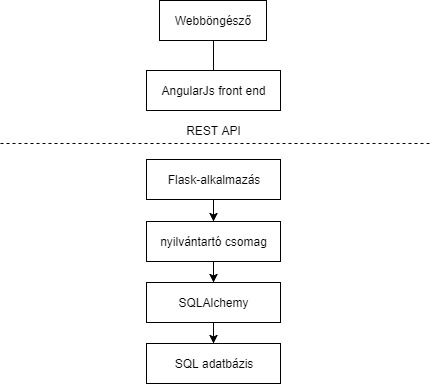
\includegraphics[scale=0.8]{kepek/architecture.jpg}
\caption{A webalkalmazás architektúrája}
\label{fig:architecture1}
\end{figure}

A felhasználó böngészőn keresztül tudja használni az alkalmazást. Az alkalmazás használója ilyenkor az AngularJs-sel kialakított úgynevezett nézeteket látja. Kliens oldalon az Angular kontrollerjei végzik a kérések elküldését a szerver irányába, melyekre a szerver az adatok visszaküldésével válaszol. A kapott válaszokat szintén az kontrollerek dolgozzák fel. A felhasználói felületről és az Angularról az ötödik fejezetben fogok bővebben írni.

% TODO: Apróság, de a fejezetet itt is majd \ref-el kellene hivatkozni!

A szerver oldalon egy többrétegű struktúrát hoztam létre. Az alsó réteg az adatbázis, ami egy SQLite alapú relációs adatbázis, amelyhez a keretrendszer SQLAlchemy ORM-en keresztül csatlakozik, tehát a lekérdezéseket az SQLAlchemy-vel végzem. Az SQL adatbázist a 4. fejezetben fogom részletesebben taglalni.

A klienstől érkező kérések feldolgozására az alkalmazás a Flask webes mikro keretrendszert használja. A flaskos réteg HTTP válaszokat küld a kliensnek, melyeben az adatok JSON formátumúak. A flaskos réteg és az alsóbb rétegek között van egy közbenső réteg, az általam készített nyilvántartó csomag. A nyilvántartó csomagban lévő metódusok végzik a lekérdezéseket, ezeket a metódusokat hívom meg a flaskos rétegben. A közbenső réteg bevezetésére a későbbi továbbfejlesztési lehetőségek miatt volt szükség. A flask és a nyilvántartó csomag bemutatására a ötödik fejezetben fog sor kerülni.

\Section{Az alkalmazás alapfunkciói}

Az alkalmazásom lényegében éttermek és rendelések adatainak nyilvántartására fog szolgálni. Ebben a fejezetben az alap funkcionalitásokat fogom tárgyalni. Az első ezek közül a regisztrációval, bejelentkezéssel, felhasználói adatok kezelésével kapcsolatosak, azt követően pedig a vásárlói és étteremtulajdonos funkciók bemutatása következik.

\bigskip

\noindent \textbf{Regisztráció/bejelentkezés}

\medskip

Az alkalmazásom egyik alap funkcionalitása a felhasználókezelés lesz. Csak regisztrált felhasználók számára lesznek elérhetőek a szolgáltatások, a kezdőlapon lesz lehetőség a bejelentkezésre vagy regisztrációra. Alapvetően két felhasználói csoportot lehet majd megkülönböztetni, a vásárlókat és az étteremtulajdonosokat. A két csoport eltérő jogosultsági körrel fog rendelkezni, és más-más szolgáltatások lesznek számukra elérhetőek.

\bigskip

\noindent \textbf{Felhasználói adatok megjelenítése}

\bigskip

A felhasználók számára lesz egy szolgáltatás, amely kilistázza az adott account adatait.

\bigskip

\noindent \textbf{Jelszó módosítás}

\bigskip

A felhasználói adatok kilistázása mellett lehetőség lesz a jelszó módosításra is. Ehhez egy űrlap kitöltésére lesz szükség, ahol meg kell majd adni az aktuális érvényben lévő jelszó mellett az új jelszót is. Az megadott adatokat szerver oldalon fogom vizsgálni, ha a megadott jelszó megegyezik a felhasználói fiók tényleges jelszavával, akkor a szerver elvégzi a szükséges adatbázis módosításokat.

\SubSection{Vásárlók funkciói}

\bigskip

\noindent \textbf{Böngészés az éttermek között}

\bigskip

A vásárlóknak lehetőségük lesz az adatbázisban szereplő éttermek kínálatai között böngészni. Szűrési feltételek megadásával szűkíthetik a kilistázott éttermek listáját, hogy megtalálják a számukra legszimpatikusabbat.

A kívánt étterem kiválasztása után a szerver kilistázza az adott étterem által kínált termékeket. A termékek között is lesz lehetőség szűrésre például típus szerint. A megrendelendő termékeket a vásárló belehelyezheti a kosárba. A kosár tartalma egy Angular változóban lesz letárolva. A kosár tartalma is módosítható lesz.

\bigskip

\noindent \textbf{Rendelés}

\bigskip

A rendelés véglegesítése előtt a vásárlónak lehetősége lesz kiválasztani a kívánt fizetési módot. Rendelés során a kosár tartalma elküldésre kerül a szervernek. A szerver létrehozza a szükséges order és \texttt{order\_meals} objektumokat, majd letárolja őket az adatbázisban. A rendelésről visszajelzést fog kapni a vásárló és az étterem tulajdonosa is. A rendelések adatait később statisztikák, kimutatások készítésénél lehet majd felhasználni.

\bigskip

\noindent \textbf{Törzsvásárlói kedvezmények}

\bigskip

A vásárlók hűségének honorálása miatt, minden leadott rendelés után jutalompontokat írunk jóvá a rendelést leadó felhasználó javára. A pontokat fizetéskor lehet majd beváltani, ilyenkor a pontok összege levonásra fog kerülni a rendelés összegéből.

\Section{Étteremtulajdonosi funkciók}

Az étteremtulajdonosoknak nyújtott szolgáltatások az éttermeik menedzselése, új éttermek felvitele a rendszerbe, és az éttermeikkel kapcsolatos statisztikák kimutatása.

\bigskip

\noindent \textbf{Éttermeim}

\bigskip

Az étterem tulajdonos számára adott lesz egy funkció, melynek segítségével ki tudják majd listázni a tulajdonukban lévő éttermeket. A felhasználó minden éttermének megtudja majd nézni a termék kínáltát, az étterembe leadott rendeléseket és tudja majd módosítani az adott étterem adatait.

\newpage

\noindent \textbf{Termékek módosítása}

\bigskip

A felhasználó minden egyes éttermének meg tudja nézni a termékkínálatát. A termékekre lesz szűrési lehetőség a köztük történő navigáció megkönnyítése érdekében. Az egyes termékeket lehet majd törölni és módosítani, illetve lesz lehetőség újabb termékek felvitelére az adatbázisba.
A termékek módosítása egy űrlap kitöltésével fog kezdődni, ahol meg kell majd adni a módosítandó adatokat. Ezeket az adatokat a szerver fogja megkapni, feldolgozni, és végrehajtani az adatbázisban.

\bigskip

\noindent \textbf{Termékek törlése}

\bigskip

A törlendő termékre a felhasználó meghívhatja a termék törlése funkciót, ekkor a termék letárolódik egy Angular változóban és elküldésre kerül a szervernek. A szerver feldolgozza a kapott adatokat, az adatbázisból törli a megfelelő azonosítójú terméket, majd véglegesíti az adatbázis módosításokat.

\bigskip

\noindent \textbf{Termék felvitel}

\bigskip

A termék felvitel funkció meghívásakor a felhasználó egy űrlapot fog látni. Miután kitöltötte a megfelelő mezőket, a felvitt adatok elküldésre kerülnek. A szerver a kapott adatokat feldolgozza, és létrehoz egy meal objektumot az adatok felhasználásával. Ezt az objektumot felviszi az adatbázisba, majd véglegesíti az adatbázis módosításokat.

\bigskip

\noindent \textbf{Étterem létrehozása}

\bigskip

A felhasználó éttermeket is hozzátud adni az adatbázishoz. Egy étterem felviteléhez mindössze egy űrlapot kell kitölteni a megfelelő adatokkal. Kitöltés után az adatokat az angular továbbítja a servernek. A server a kapott adatokból létrehoz egy új restaurant objektumot, és menti az adatbázisba.

\bigskip

\noindent \textbf{Étterem módosítsa}

\bigskip

Egy étterem módosításához egy űrlap kitöltésére lesz szükség, amire a módosítandó adatokat kell felvinni. Az űrlap elküldése után az Angular továbbítja az adatokat a szervernek, ami feldolgozza és véglegesíti a módosításokat.

\bigskip

\noindent \textbf{Rendelések}

\bigskip

A felhasználó mindegyik éttermére megtudja majd hívni a rendelések funkciót, amely kilistázza az adott étteremben leadott rendeléseket.

\newpage

\noindent \textbf{Statisztikák}

\bigskip

Az étterem tulajdonosok számára lesz egy szolgáltatás, amely statisztikákat, grafikonokat állít elő egy adott időszakra, melyek nélkülözhetetlenek a további üzleti lépések meghozatalához, a sikeres üzleti élethez. A felhasználók megnézhetik például, hogy melyik ételtípusból rendelik a legtöbbet, a különböző fizetési módok gyakoriságát, vagy például a felhasználók rendelésszámának eloszlását.


\chapter{A rendelések adatainak nyilvántartása}

%Itt magáról az adatmodellről van szó gyakorlatilag. Itt érdemes kifejteni, hogy milyen adat, és hol kerül majd tárolásra. Az ER jellegű diagram, illetve az SQLAlchemy-s modellek egyszerűsített változata kellene majd ide.

%A rendelések adatainak nyilvántartása
Az adatbázis tervezése során az egyik fő célom az volt, hogy könnyen módosítható, illetve kibővíthető legyen a rendszer. Első lépésként a fontosabb egyedeket határoztam meg, majd a köztük lévő kapcsolatokat. A dolgozatom készítése során elkészítettem két kezdetleges adatmodellt, amelyeknek az összefésüléséből megszületett a végleges adatmodell. Az alkalmazás implementálása során számos alkalommal kellett módosítanom az adatbázist.

Az általam tervezett adatmodell egyes táblái és a köztük lévő kapcsolatok \aref{fig:rendeles_sema} ábrán láthatók.

\begin{figure}
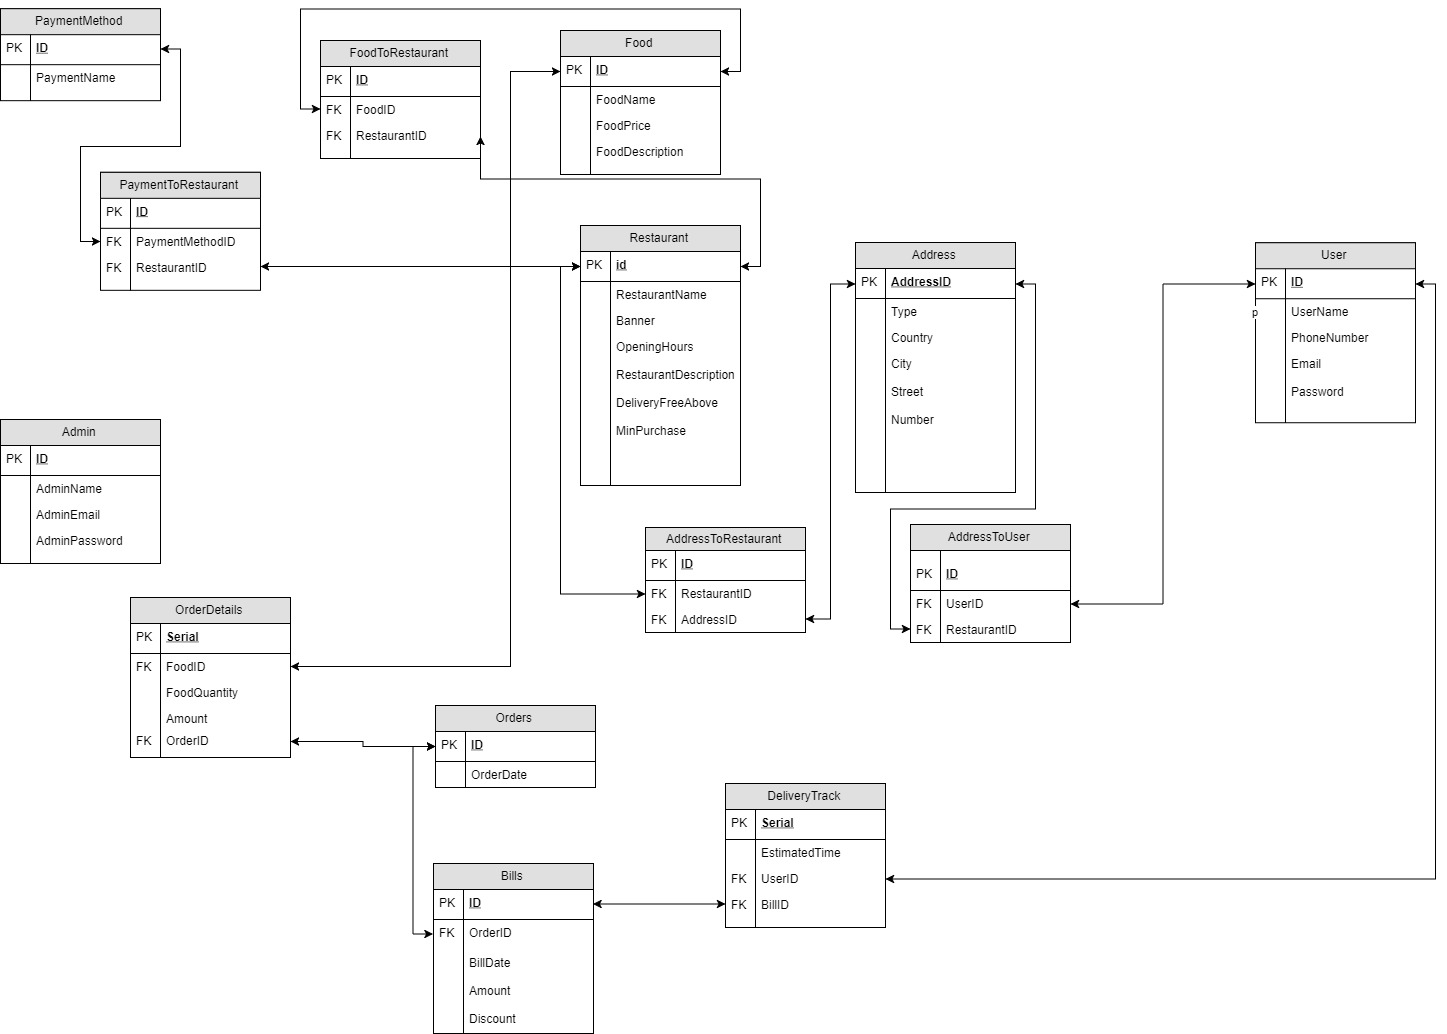
\includegraphics[scale=0.3]{kepek/rendeles_sema.jpg}
\caption{A rendelések adatait kezelő adatábis sémája}
\label{fig:rendeles_sema}
\end{figure}

\section{users}

Az online alkalmazásomon keresztül való étel rendeléshez regisztrált felhasználónak kell lenni. Ez a tábla a regisztrált felhasználókról tartalmaz információkat, illetve az adatbázisban lévő éttermek tulajdonosairól. Minden felhasználó rendelkezik egy azonosítóval, egy kereszt egy vezeték és egy felhasználónévvel, jelszóval továbbá egy telefonszámmal, egy email címmel. Mindegyikhez tartozik egy address, illetve abban az esetben a felhasználó típusa 1-es, - tehát étterem tulajdonos - akkor tartozik hozzá egy restaurant.

\begin{tabular}{|p{3cm}|p{10cm}|}
\hline
user\_id & Elsődleges kulcs, a felhasználó azonosítója. \\
\hline
first\_name & A regisztrált felhasználó keresztneve. \\
\hline
last\_name & A regisztrált felhasználó vezetékneve. \\
\hline
user\_name & A regisztrált felhasználó felhasználóneve. \\
\hline
password & A felhasználó jelszava. \\
\hline
phone\_number & A felhasználó telefonszáma. \\
\hline
email & A felhasználó email címe. \\
\hline
user\_role & Felhasználó típus, lehetséges értékek: 0: egyszerű felhasználó 1: étterem tulajdonos \\
\hline
\end{tabular}

\section{restaurants}

Ez a tábla tartalmazza az éttermeket és a hozzájuk tartozó információkat. A tábla minden bejegyzéséhez tartozik egy address, illetve minden étteremhez tartozik egy user is. Egy étteremhez tartozik egy azonosító, egy név, egy leírás étteremről, meg kell adni az étteremből való rendelés minimális összegét továbbá a kiszállítás maximális időtartamát. Opcionálisan tartalmazhatja a kiszállítás árát, a kiszállítás minimális idejét illetve az étterem logójának URL címét.
Kötelező mezők

\begin{tabular}{|p{3cm}|p{10cm}|}
    \hline
    restaurant\_id & Elsődleges kulcs, az étterem azonosítója. \\
    \hline
    restaurant\_name & Az étterem neve. \\
    \hline
    restaurant\_description & Az étterem leírása. \\
    \hline
    min\_order & Az étteremből való rendelés minimális összege. \\
    \hline
    delivery\_max\_time & Az étteremből való kiszállítás maximális időtartama. \\
    \hline
\end{tabular}

\section{meals}

Ebben a táblában tárolom az adott éttermek által forgalmazott ételeket, italokat. A táblának egy bejegyzése egy étteremhez tartozik, de egy adott étteremhez több meal is tartozhat. A táblában minden bejegyzéshez tartozik egy azonosító, egy név, egy leírás, a termék ára, a terméket forgalmazó étterem azonosítója illetve opcionálisan meg lehet adni a termék logójának URL címét.
Kötelező mezők

\begin{tabular}{|p{3cm}|p{10cm}|}
    \hline
    meal\_id & Elsődleges kulcs, a termék azonosítója \\
    \hline
    meal\_name & Az étel neve. \\
    \hline
    meal\_description & Az étel leírása \\
    \hline
    meal\_price & Az étel ára. \\
    \hline
    restaurant\_id & Idegen kulcs, a terméket forgalmazó étterem azonosítója. \\
    \hline
\end{tabular}

\section{addresses}

Az addresses tábla tartalmazza a felhasználók és az éttermek címéhez tartozó információkat. Mindegyik vagy egy étteremhez vagy egy felhasználóhoz tartozik, egy felhasználóhoz több cím is tartozhat. Egy címhez mindig tartozik egy azonosító, egy típus(szállítási, vagy lakcím), egy város, utca illetve házszám, továbbá vagy egy étterem vagy egy felhasználó azonosító attól függően, hogy étteremhez vagy felhasználóhoz tartozik e a cím.
Kötelező mezők

\begin{tabular}{|p{3cm}|p{10cm}|}
    \hline
    address\_id & Elsődleges kulcs, a cím azonosítója. \\
    \hline
    address\_type & A cím típusa, értéke lehet: 0: lakcím 1: szállítási cím \\
    \hline
    address\_city & A cím város komponense. \\
    \hline
    address\_street & A cím utca komponense. \\
    \hline
    address\_number & A cím házszám komponense. \\
    \hline
    restaurant\_id & Idegen kulcs, a címhez tartozó étterem azonosítója \\
    \hline
    user\_id & Idegen kulcs, a címhez tartozó felhasználó azonosítója \\
    \hline
\end{tabular}

\section{orders}

Ez a tábla tartalmazza a rendeléseket. Egy rendeléshez order\_meal-ek tartoznak, ezek tartalmazzák a megrendelt termékek adatait. Minden rendelés tartalmaz egy azonosítót, egy dátumot, egy árat, illetve a rendelést leadó felhasználó azonosítóját.
Kötelező mezők

\begin{tabular}{|p{3cm}|p{10cm}|}
\hline
order\_id & Elsődleges kulcs, a rendelés azonosítója. \\
\hline
order\_date & A rendelés dátuma. \\
\hline
order\_price & A rendelés összege. \\
\hline
user\_id & A rendelést leadó felhasználó azonosítója \\
\hline
\end{tabular}

\section{order\_meals}

Ez a tábla a felhasználó által kosárba helyezett termékekről tartalmaz információkat. Egy order\_meal bejegyzés egy megrendelt termékről tárol adatokat. Minden bejegyzés tartalmaz rendelés azonosítót, ami megadja, hogy egy order\_meal melyik rendeléshez tartozik. Egy rendeléshez több order\_meal is tartozhat. Mindegyeik order\_meal-hez tartozik az rendelés azonosítón kívül egy azonosító, egy darabszám, egy ár, illetve egy termék azonosító.
Kötelező mezők

\begin{tabular}{|p{3cm}|p{10cm}|}
    order\_meals\_id & Elsődleges kulcs, az order\_meal azonosítója. \\
    \hline
    order\_meals\_quantity & A megrendelt termék darabszáma. \\
    \hline
    order\_meals\_price & A megrendelt termék ára. \\
    \hline
    order\_id & Idegen kulcs, a rendelés azonosítója, amihez az order\_meal tartozik. \\
    \hline
    meal\_id & Idegen kulcs, az order\_meal-hez tartozó termék azonosítója. \\
    \hline
\end{tabular}

\section{payments}

Ebben a táblában az éttermek által biztosított fizetési lehetőségeket tárolom. Minden bejegyzéséhez tartozik egy étterem azonosító, amivel meg lehet adni, hogy az adott fizetési lehetőségek melyik étteremhez tartoznak. Egy ilyen bejegyzés tartalmazza az imént említett étterem azonosítót, továbbá egy azonosítót, és különböző fizetési lehetőségeket, melyeknek az értéke 0, ha az adott étteremnél nem lehet ilyen módon fizetni, illetve 1 ha lehet.

\begin{tabular}{|p{3cm}|p{10cm}|}
    payment\_id & Elsődleges kulcs, a payment azonosítója. \\
    \hline
    cash & Készpénzes fizetési lehetőség. \\
    \hline
    creditcard & Bankkártyás fizetési lehetőség. \\
    \hline
    szep\_card & SZÉP kártyás fizetési lehetőség. \\
    \hline
    erzsebet\_voucher & Erzsébet utalvány elfogadása. \\
    \hline
    restaurant\_id & Idegen kulcs, az étterem azonosítója, amelyikhez tartozik az adott payment. \\
    \hline
\end{tabular}

\section{Back-End}

A szerver oldalon egy többrétegű struktúrát hoztam létre. Ebben a fejezetben a két felső réteget, a Flask alkalmazást és a nyilvántartó csomagot fogom részletezni

\subsection{Nyilvántartó csomag}

A nyilvántartó csomagban lévő metódusok végzik a lekérdezéseket, ezeket a metódusokat hívom meg a flaskos rétegben. A nyilvántartó csomag egy absztrakciós szintet biztosít, elfedi az alsóbb rétegek technikai részleteit. A közbenső réteg bevezetésének számos előnye volt. Rövidebb és átláthatóbb lett a Flask fájl, mivel a lekérdezések, ellenőrzések és eredmények feldolgozására átkerült a nyilvántartó csomag függvényeibe. Így a Flask szinte csak a paraméterek lekérdezésével és a válaszok előállításával foglalkozik.

A nyilvántartó csomag egyik legnagyobb előnye a későbbi továbbfejlesztési lehetőségekben rejlik. Ha a későbbiekben szeretnék egy mobil vagy asztali alkalmazást csinálni, csupán a Flaskos réteget kellene lecserélni, a back-end többi része maradhatna.

A nyilvántartó library 6 pyton fájlt tartalmaz, melyekben különböző függvények lettek implementálva. A további ezeket a fájlokat és függvényeket fogom ismertetni.

\subsection{\texttt{Adddress.py}}

\begin{itemize}
    \item \texttt{query\_cities()}: Az adatbázisban található éttermekhez rendelt címeket kérdezi le. Dictionary-k listájaként a címek város komponensét adja vissza.
\end{itemize}

\subsection{\texttt{Meal.py}}

\begin{itemize}
    \item \texttt{query\_meals(restaurant\_id)}:
        Az adatbázisból a paraméterként megadott azonosítójú étterem kínálatában lévő ételeket kérdezi le, az eredmény dictionary-k listájaként adja vissza.
    \item \texttt{query\_meal\_types(restaurant\_id)}:
        A paraméterként kapott étterem kínálatában lévő ételek típusait kérdezi le az adatbázisból, az eredményt ez a függvény is dictionary-k listájaként adja vissza.
    \item \texttt{add\_new\_meal(newMeal)}:
        A paraméterként kapott adatokból létrehoz egy új Meal objektumot, és azt menti az adatbázisban.
    \item \texttt{remove\_meal(removable\_meal)}:
        Az adatbázisból lekérdezi a paraméterként kapott Meal objektum azonosítójával megegyező azonosítójú ételt, és azt törli az adatbázisból. Törlés után véglegesíti az adatbázis módosításokat.
    \item \texttt{query\_meal\_data\_by\_id(meal\_id)}:
        Paraméterként kap egy étel azonosítót. Lekérdezi az adatbázisból a kapott azonosítóval megegyező azonosítójú ételt, a kapott eredményt a függvény dictinary-ként adja vissza.
    \item \texttt{edit\_meal(params)}:
        Ez a függvény kerül meghívásra, amikor egy adatbázisban lévő étel adatait akarjuk módosítani. Paraméterként kap egy étel azonosítót, egy étterem azonosítót, és a módosítandó adatokat. A kapott étel azonosítóval megegyező azonosítójú ételt lekérdezi az adatbázisból, az adatmódosításokat elvégzi, és véglegesíti az adatbázis módosítást. A status nevű változóval tér vissza, melynek értéke sikeres módosítása esetén 200, sikertelen esetén 401.
    \item \texttt{query\_meal\_type\_stat(username, restaurant\_id)}:
        A paraméterként kapott felhasználónévvel megegyező felhasználónevű user-t lekérdezi az adatbázisból. A Meal táblából lekérdezi azokat az ételeket étel típus szerint csoportosítva, amiknek az étterem azonosítójuk megegyezik a paraméterként kapott azonosítóval. Az Order adatbázis táblából lekérdezi azokat a rendeléseket, melyeknél az étterem azonosító megegyezik a kapott azonosítóval. A lekérdezések eredményének segítségével összeszámolja, hogy a paraméterként kapott azonosítóval rendelkező étteremben leadott rendelésekben hány darab van a különböző ételtípusokból. Az eredményt a függvény dictionary-k listájaként adja vissza.
\end{itemize}

\subsection{\texttt{Order.py}}

\begin{itemize}
\item \texttt{checkout\_order(newOrder)}:
Lekérdezi az adatbázisból a paraméterként kapott azonosítójú ételt, és a kapott felhasználónévvel megegyező felhasználónevű usert. Létrehoz egy új rendelés objektumot a paraméterként kapott, és a lekérdezett értékekből. Az adatbázis mentése előtt módosítja a felhasználó jutalompontjainak a számát egy képlet alapján. A függvény még létrehoz egy Order\_meals objektumot is a paraméterként kapott adatokból. Ezeket az adatbázis műveleteket is véglegesíti. Amennyibben minden sikeres volt a függvény visszatér a status változóval, melynek 200-ra állítja be az értékét.
\item \texttt{query\_orders()}:
Lekérdezi az adatbázisban található összes rendelést, az eredményt dictionary-k listájaként adja vissza.
\item \texttt{query\_my\_orders(username, restaurant\_id)}:
Az adatbázisból lekérdezi a paraméterként kapott felhasználónévvel megegyező nevű felhasználót, és a kapott étterem azonosítóval egyező azonosítójú éttermet. Továbbá lekérdezi az Order táblából azokat a rendeléseket, melyeknek az étterem azonosítója megegyezik a kapott azonosítóval. A lekérdezések eredményéből összeállít egy listát, amiben dictionary-k vannak tárolva, és ezt adja vissza eredményként.
\end{itemize}

\subsection{\texttt{Payment.py}}

\begin{itemize}
\item \texttt{query\_payments(restaurant\_id)}:
Lekérdezi az adatbázisból azokat a fizetési módokat, melyeknek az étterem azonosítójuk megegyezik a paraméterként kapottal. A kapott eredményen végig iterál egy for ciklussal, amelyik fizetési mód értéke 1, ahhoz hozzá rendeli a Payment nevű enum osztályból a megfelelő értéket. A függvény egy listával tér vissza, amiben dictionary-k vannak.
\item \texttt{query\_payment\_type\_stat(username, restaurant\_id)}: 
A paraméterként kapott felhasználónévvel megegyező felhasználónevű user-t lekérdezi az adatbázisból. A PaymentTable táblából azt a bejegyzést, amelyiknek az étterem azonosítója megegyezik a paraméterben kapottal. A függvény összeszámolja, hogy az adott étteremben leadott rendelések során milyen gyakorisággal választották az egyes fizetési módokat. Az eredményt dictionary-k listájaként adja vissza.
\end{itemize}

\subsection{\texttt{Restaurant.py}}

\begin{itemize}
\item \texttt{query\_restaurants()}:
Az adatbázisban lévő összes éttermet lekérdezi, az eredményt dictionary-k listájaként adja vissza.
\item \texttt{query\_my\_restaurants(current\_username)}:
A paraméterként kapott felhasználónévvel megegyező felhasználónevű usert lekérdezi a User táblából. Restaurant táblából lekérdezi azokat az éttermeket, melyek felhasználó azonosítója megegyezik a lekérdezed felhasználó azonosítójával. Az eredmény dictionary-k listájában adja vissza.
\item \texttt{query\_restaurant\_by\_name(newRestaurant)}:
A függvény az adatbázisból lekérdezi a paraméterben kapott névvel megegyező nevű éttermet, és azt adja vissza eredményként.
\item \texttt{add\_new\_restaurant(newRestaurant)}:
A paraméterként kapott felhasználónévvel megegyező nevű felhasználót lekérdezi. Létre hozz egy új étterem objektumot a paraméterben kapott, és a lekérdezett adatokból. Felviszi az új éttermet az adatbázisba, és véglegesíti az adatbázismódosításokat. Egy új cím objektumot is létrehoz, szintén a paraméter adatokból, és felviszi az adatbázisba. Az új cím objektumhoz hozzárendeli az új étterem azonosítóját.
\item \texttt{query\_restaurant\_by\_id(params)}:
A paraméterként megadott azonosítójú éttermet adja vissza.
\item \texttt{edit\_restaurant(params, restaurant)}:
Lekérdezi azt a felhasználót, amelyikhez hozzá van rendelve a paraméterként kapott azonosítójú étterem. Ellenőrzi, hogy a paraméterben kapott jelszó megegyezik e lekérdezett felhasználó jelszavával, ha igen akkor elvégzi a módosításokat, menti az adatbázist, a status változott 200-ra állítja, és visszatér vele. Amennyiben a két jelszó nem egyezik, a status változó értéke 401 lesz, és azzal tér vissza.
\item \texttt{query\_my\_restaurant\_data(restaurant\_id)}:
Az adatbázisból lekérdezi a paraméterként kapott azonosítójú éttermet, és a hozzárendelt címet. Az adatokat egy dictionary-ben adja vissza.
\end{itemize}

\subsection{\texttt{User.py}}

\begin{itemize}
    \item \texttt{query\_user\_by\_name(newUser)}:
A paraméterként kapott felhasználónevű felhasználót lekérdezi, és visszatér vele.
\item \texttt{user\_registration(newUser)}:
A paraméterként kapott adatokból létrehoz egy új User objektumot, és menti az adatbázisban. Egy Address objektumut is létrehoz a kapott adatokból, és hozzá rendeli a létrehozott felhasználót. 
\item \texttt{query\_users()}:
Az adatbázisban lévő összes felhasználót lekérdezi, és egy dictionary-ket tartalmazó listában adja vissza őket.
\item \texttt{edit\_user(params)}:
A paraméterként kapott felhasználónevű felhasználót lekérdezi, majd ellenőrzi, hogy a paraméterként kapott jelszó egyezik e a lekérdezett felhasználó jelszavával. Ha egyezik módosítja a felhasználó jelszavát, menti az adatbázist, status változót 200-ra állítja és visszatér vele. Amennyiben nem egyezik a status változót 401-re állítja, és visszatér vele.
\item \texttt{query\_user\_data(username)}:
A paraméterként kapott felhasználónevű felhasználót lekérdezi, majd a hozzá tartozó címeket is. A kapott eredményeket dictionary-k listájában adja vissza.
\item \texttt{user\_login(current\_user)}:
Lekérdezi az adatbázisban található összes felhasználót, majd egy for ciklussal végig iterál a kapott eredményen. A ciklus magban vizsgálja, hogy a paraméterként kapott felhasználónévvel talál e megegyezőt, ha igen, akkor megvizsgálja a szintén paraméterként kapott jelszó helyességét is. Deklarál egy payload dictionary-t a felhasználónévből, azonosítóból és egy generált számsorból. A JWT encode függvényének meghívásával létrehoz egy tokent, az encode paraméterként megkapja a payload-ot és egy titkos kulcsot. Az autentikációhoz szükséges adatokat a login\_user dictionary-ban tárolja, és sikeres azonosítás esetén ezzel tér vissza. Sikertelen bejelentkezés esetén a status változó értékét 202-re állítja és azzal tér vissza.
\end{itemize}

\section{Flask webalkalmazás}

A klienstől érkező kérések feldolgozására az alkalmazás a Flask webes mikro keretrendszert használja. A flaskos réteg http válaszokat küld a kliensnek, melyeben az adatok JSON formátumúak. A flaskos réteg és az alsóbb rétegek között van egy közbenső réteg, az általam készített nyilvántartó csomag. A nyilvántartó csomagban lévő metódusok végzik a lekérdezéseket, ezeket a metódusokat hívom meg a flaskos rétegben. A közbenső réteg bevezetésére a későbbi továbbfejlesztési lehetőségek miatt volt szükség. A flask és a nyilvántartó csomag bemutatására a hetedik fejezben fog sor kerülni.

A flaskos réteg a kliens oldalról érkező kérések feldolgozását végzi. Amennyiben a kapott kérésben volt paraméter, megvizsgálja annak helyeségét. A válaszhoz szükséges adatok előállítását a nyilántartó csomag végzi, a flaskos rétegben csak meg kell hívni a megfelelő metódusokat a szükséges paraméterezéssel. Az előállított adatokból létrehozza a választ, és JSON formátumban továbbítja a kliensnek.

\subsection{\texttt{Index.py}}

Az index.py fájlban van implementálva a flaskos réteg. Minden flaskos függvény a route() dekorátorral van ellátva, ez a dekorátor azt írja le, hogy melyik URL-re hivatkozza fog meghívódni az adott függvény.

A továbbiakban az útvonalakat és a hozzájuk tartozó \textit{endpoint} függvényeket fogom részletezni.
A függvények neve és URL címek (\textit{az index függvény kivételével}) megegyeznek, ezért az alpontok címénék mindig az adott függvény URL-jét fogom megadni.

\begin{itemize}
\item \texttt{/}:
Az index() függvény meghívása a „/” URL-re hivatkozva történik. Ez az alkalmazás megnyitásakor és főoldal gombra való kattintáskor fordul elő, ilyenkor elküldi az index.html fájlt.
\item \texttt{/registration}:
Új felhasználót visz fel az adatbázisba. Először lekérdezi a paraméterben kapott felhasználónevű usert, megvizsgálja, hogy foglalt e már ez a felhasználónév. A lekérdezéshez a query\_user\_by\_name() függvényt használja a newUser paraméterrel, melyben a regisztrálni kívánt felhasználó adatai vannak. Ha foglalt a felhasználónév, akkor a 409-es hibakóddal tér vissza. Ha nem foglalt, meghívja a user\_registration() függvényt szintén a newUser paraméterrel, a függvény elvégzi a szükséges adatbázisműveleteket, majd visszatér a registration() metódushoz, ami 200-as státuszkódot küld válaszként a kliens oldalra.
\item \texttt{/checkout}:
Ez a függvény rendelések leadásakor/kifizetésekor kerül meghívásra. Flaskos oldalon csak a checkout\_order() metódus meghívása történik a newOrder paraméterrel. A newOrderben a rendeléshez szükséges adatok vannak, ezeket a meghívott függvény feldolgozza és visszatér egy státusz kóddal. A checkout() függvény a kapott státuszkódot küldi el kliensnek válaszként.
\item \texttt{/users}:
Az adatbázisban található összes felhasználót lekérdezi, és egy JSON fájlban küldi el a kliens oldalra. A lekérdezéshez a query\_users() függvényt használja.
\item \texttt{/login}:
A login() függvény bejelentkezéskor kerül meghívásra, ez végzi az autentikációt. Meghívja a user\_login() metódust a current\_user paraméterrel. A metódus visszatérési értékét vizsgálja, ha az értéke 202, akkor hiba lépett fel az autentikáció közben, és a 202-es státuszkódot küldi válaszul a kliensek. Ha nem egyenlő 202-vel, akkor az autentikáció sikeres volt, a kliensnek elküldi a user\_login() visszatérési értékét és egy 200-as státuszkódot.
\item \texttt{/restaurants}:
Az adatbázisban található összes éttermet lekérdezi, a kapott eredményt JSON formátumban továbbítja a kliens oldalra. A lekérdezéshez a query\_restaurants() függvényt használja.
\item \texttt{/myRestaurant}:
A paraméterként kapott felhasználó tulajdonában lévő éttermek listáját küldi a kliensnek. A lekérdezéshez a query\_my\_restaurants() metódust hívja meg a current\_username paraméterrel. A current\_username a bejelentkezett felhasználó nevét tárolja.
\item \texttt{/meals}:
A paraméterként kapott étterem által kínált étel kínálatot továbbítja a kliens felé. A lekérdezést a query\_meals() metódus végzi restaurant\_id-val paraméterezve.
\item \texttt{/orders}:
Az adatbázisban lévő összes leadott rendelést kérdezi le, és küldi el JSON formátumban a kliens oldalra. A query\_orders() metódus végzi a lekérdezést.
\item \texttt{/cities}:
Lekérdezi azokat a városokat, melyekben található az adatbázisban szereplő étterem, az eredményt továbbítja a kliens oldalra. A lekérdezéshez a query\_cities() metódust hívja meg.
\item \texttt{/types}:
A paraméterként kapott étterem kínálatában lévő ételtípusokat kérdezi le és küldi el a kliens részére. A query\_meal\_types() metódust restaurant\_id-vel paraméterezve használja a lekérdezéshez.
\item \texttt{/payments}:
A paraméterként kapott étterem által kínált fizetési módokat kérdezi le, és küldi el válaszként a kliens oldalra. Lekérdezéshez a query\_payments() függvényt használja restaurant\_id-val paraméterezve.
\item \texttt{/addRestaurant}:
A paraméterként kapott adatokból létrehoz egy új étterem objektumot, és felviszi az adatbázisba. Első lépésként a newRestaurant-al paraméterezett query\_restaurant\_by\_name() metódussal lekérdezi, az adatbázisból, hogy van e már a paraméterben megadottal megegyező nevű étterem. A lekérdezett eredményt a flaskos oldalon vizsgálom, ha van már ilyen, akkor a függvény 409-es státuszkóddal tér vissza a kliens oldalra. Amennyiben nem volt még ilyen nevű étterem meghívásra kerül az a add\_new\_restaurant() a newRestaurant paraméterrel, és elvégzi a szükséges adatbázisműveleteket. Sikeres felvitel eseten az addRestaurant() 200-as státuszkódot küld a kliensnek.
\item \texttt{/addMeal}:
A paraméterként kapott adatokból létrehoz egy új étel objektumot, és felviszi azt az adatbázisba. A newMeal-el paraméterezett add\_new\_meal() metódus hajtja végre a szükséges műveleteket. Sikeres adatbázisműveletek eseten 200-as státuszkódot küld válaszként a kliensnek.
\item \texttt{/removeMeal}:
A paraméterként kapott ételt törli az adatbázisból. A törlést a remove\_meal() függvény végzi, paraméterezni kell a függvényt a törlendő étellel. Sikeres törlés esetén 200-as státuszkódot küld válaszként.
\item \texttt{/myOrders}:
A paraméterként kapott éteremben leadott összes rendelést kérdezi le, és továbbítja a kliens oldalra. A lekérdezéseket a query\_my\_orders() függvény végzi. A függvényt a username, és a restaurant\_id paraméterekkel kell meghívni. Sikeres lekérdezések után a lekérdezés eredményét küldi el válaszként JSON formátumban.
\item \texttt{/userData}:
A jelenleg bejelentkezett felhasználó felhasználói adatait kérdezi le, a lekérdezett eredményt küldi válaszként a kliensnek. A lekérdezéshez a query\_user\_data() függvényt hívja meg username paraméterrel.
\item \texttt{/editUser}:
Lekérdezi a paraméterként kapott felhasználó adatait, ellenőrzi, hogy a paraméterként kapott jelszó megegyezik e a lekérdezett felhasználó jelszavával, ha igen akkor az adatbázisban módosítja a felhasználó jelszavát. Az params paraméterrel ellátott és meghívott edit\_user() metódus végzi a lekérdezéseket, ellenőrzést, és az adatbázisműveleteket. Sikeres jelszó módosítás esetén 200-as státuskódot küld válaszként a kliensnek.
\item \texttt{/restaurantData}:
A paraméterként kapott étterem adatait módosítja a szintén paraméterként kapott adatok alapján, majd véglegesíti az adatbázismódosításokat. Sikeres adatmódosítás esetén 200-as státuszkódot küld a kliensnek. A kapott étterem azonosítót paraméterként adja a query\_restaurant\_by\_id() függvénynek, így lekérdezi a szükséges étterem objektumot az adatbázisból. A params, és restaurant paraméterekkel meghívott edit\_restaurant() metódus pedig elvégzi az ellenőrzéseket és az adatbázisműveleteket.
\item \texttt{/mealData}:
Lekérdezi a paraméterként kapott étel adatait, a kapott adatokat küldi válaszként a kliensnek. A lekérdezést a meal\_id paraméterrel ellátott query\_meal\_data\_by\_id() metódus végzi.
\item \texttt{/editMeal}:
Paraméterként kapott adatokkal módosítja egy étel adatait. A paraméterként kapott étel azonosítóval rendelkező ételt lekérdezi, lekérdezi az éttermet, amelyik az ételt forgalmazza, és a felhasználót, akié az étterem. Egy jelszó ellenőrzés után módosítja az adatokat. Az editMeal() függvényben meghívásra kerül az edit\_meal() metódus a params paraméterrel, amely elvégzi a fentebb említett műveleteket. Sikeres adatmódosítás esetén 200-as, sikertelen esetén pedig 401-es státuszkódot küld válaszként.
\item \texttt{/editRestaurant}:
A paraméterként kapott étterem azonosítóval rendelkező éttermet lekérdezi az adatbázisból, majd a szintén paraméterként kapott adatokkal módosítja azt. Az étterem lekérdezéséhez a query\_restaurant\_by\_id(params) metódust hívja meg az itt látható paraméterezéssel. Az adatbázisműveletek és ellenőrzések elvégzéséhez pedig az edit\_restaurant() függvény kerül meghívásra a params, és a restaurant paraméterekkel. Sikeres adatmódosítás esetén 200-as, sikertelen esetén pedig 401-es státuszkódot küld válaszként.
\item \texttt{/paymentTypeStat}:
Lekérdezi, hogy a paraméterként kapott étteremben leadott rendeléseknél a különböző fizetési módok milyen gyakorisággal voltak használva. A lekérdezéseket és a lekérdezett adatok feldolgozását a query\_payment\_type\_stat() metódus végzi, ami username és restaurant\_id paraméterekkel kerül meghívásra. A kapott eredményt fogja tartalmazni a kliensnek küldött válasz.
\item \texttt{/mealTypeStat}:
Lekérdezi, hogy a paraméterként kapott étteremben leadott rendeléseknél milyen gyakorisággal rendelték a különböző ételtípusokat. Username, és restaurant\_id paraméterekkel meghívásra kerül a query\_meal\_type\_stat() metódus, ami elvégzi a lekérdezéseket, és a lekérdezett adatok feldolgozását. A kliens részére megfogalmazott válasz a lekérdezések eredményét fogja tartalmazni.
\end{itemize}

\chapter{A felhasználói felület}

Itt kellene majd bemutatni, hogy a felhasználói felület egyáltalán milyen részekből áll, azokat hogy lehet elérni és használni.

Attól függően, hogy a funkciók inkább kliens vagy szerver oldalon lesznek majd, itt lehet részletezni az összes, felhasználói felülettel kapcsolatos tudnivalót, de az is jó megoldás, ha minden funkciónál külön kerül bemutatásra.

\section{Felhasználói felület}

\subsection{Bejelentkezés/ regisztráció}

Az alkalmazás használatához érvényes felhasználói fiókra van szükség. Az alkalmazást használó felhasználókat két típusra lehet bontani, vannak az egyszerű userek(vásárlók), akik ételeket tudnak rendelni az adatbázisban szereplő éttermekből, és vannak az étteremtulajdonosok, akik saját éttermüket tudják menedzselni. Az alkalmazás további szolgáltatásainak az igénybevételéhez mindenképp be kell jelentkezni vagy userként, vagy étteremtulajdonosként. Amennyibben a felhasználó most először látogatott el az oldalra, és még nincs felhasználói fiókja, van lehetősége userként regisztrálnia magát. Ehhez mindössze egy egyszerű űrlapot kell kitöltenie, ahol többek között meg kell adnia a nevét, elérhetőségét, címét. Abban az esetben, ha valaki étteremtulajdonosként szeretne regisztrálni, meg kell keresni egy email-el az oldal üzemeltetőjét.

\begin{figure}
\centering
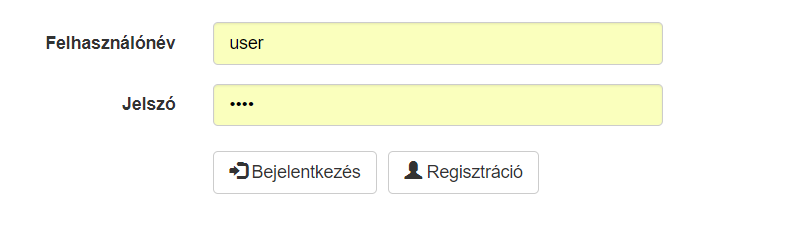
\includegraphics[scale=0.8]{kepek/login.png}
\caption{Bejelentkező felület}
\label{fig:architecture}
\end{figure}

\section{Egyszerű user funkciói}

A továbbiakban az alapfunkciókat a szerint fogom leírni, hogy melyik felhasználói csoport számára érhetők el. A vásárlók által elérhető szolgáltatásokkal kezdem

\subsection{Éttermek listázása}

A vásárlók számára adott egy olyan funkció, hogy ki tudják listázni az adatbázisban szereplő összes éttermet. Az éttermek egymás alatt, egy táblázatban jelennek meg. A táblázatban szerepel az étterem logója, neve, rövid leírása, címe, a várható kiszállítási idő, kiszállítási költség, a minimális rendelés összege és egy gomb, amire kattintva az oldal tovább irányítja a vásárlót az adott étterem étlapjához (\ref{fig:restaurants}. ábra).

A vásárlónak lehetősége van szűrni az éttermeket város szerint, ami segíti őket abban, hogy csak a számukra elérhető távolságban levő éttermek kínálatát lássák.

\begin{figure}
\centering
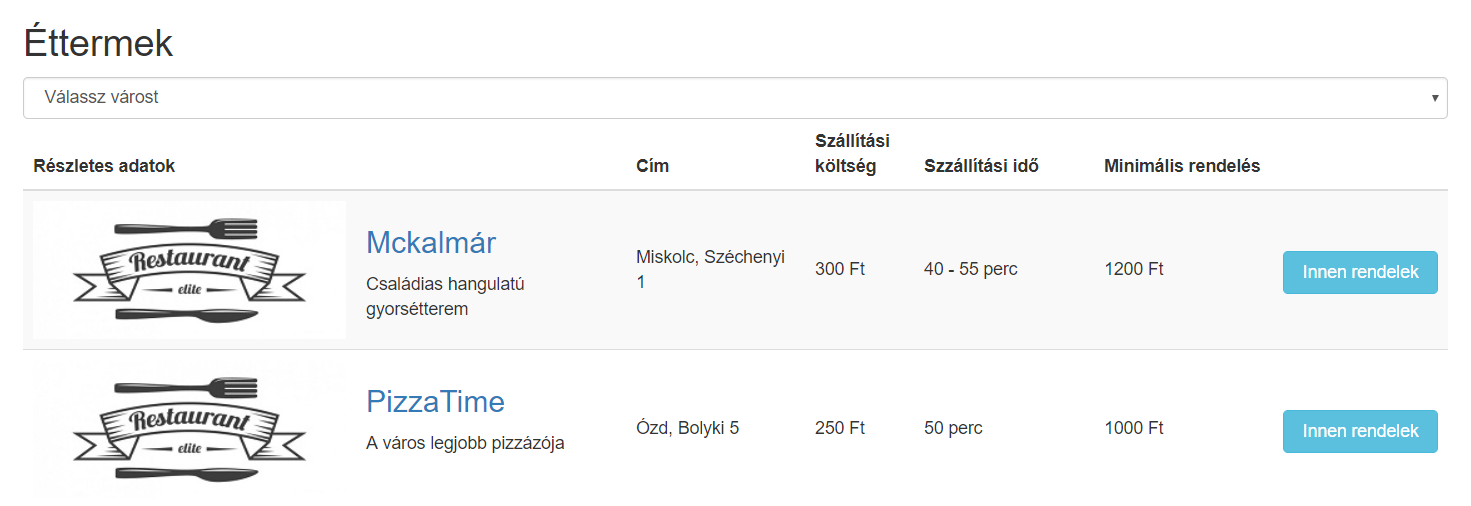
\includegraphics[scale=0.5]{kepek/restaurants.png}
\caption{Az éttermek listázása}
\label{fig:restaurants}
\end{figure}

\subsection{Étlap}

Miután a vásárló kiválasztotta a neki legszimpatikusabb éttermet, az „innen rendelek” gombra kattintva el lehet érni az adott étterem étlapját.

Az ételek egymás alatt, egy táblázatban jelennek meg (\ref{fig:menu}. ábra). A táblázat egyes soraiban egy-egy étel szerepel, az oszlopaiban pedig az adott étel adatai, többek között neve, egy kép róla, az ára és egy rövid leírás róla. A táblázat jobb szélső oszlopában egy „kosárba” feliratú gomb található, amit megnyomva a kiválasztott termék belekerül a felhasználó kosarába.

Az étlap felett van egy legördülő menü, ahol vásárló kiválaszthatja, hogy milyen típusú ételek között szeretne válogatni, milyen típusút szeretne rendelni. Az étel típus kiválasztása után, az ételek listája szűrve lesz az adott típus szerint, tehát csak a kívánt típusú ételek fognak megjelenni a táblázatban.

Miután a vásárló kiválasztotta a rendelni kívánt termékeket, és hozzáadta őket a kosárhoz, megjelenik a felületen a „fizetés” gomb, amire kattintva elérjük a fizetés funkciót.

\begin{figure}
\centering
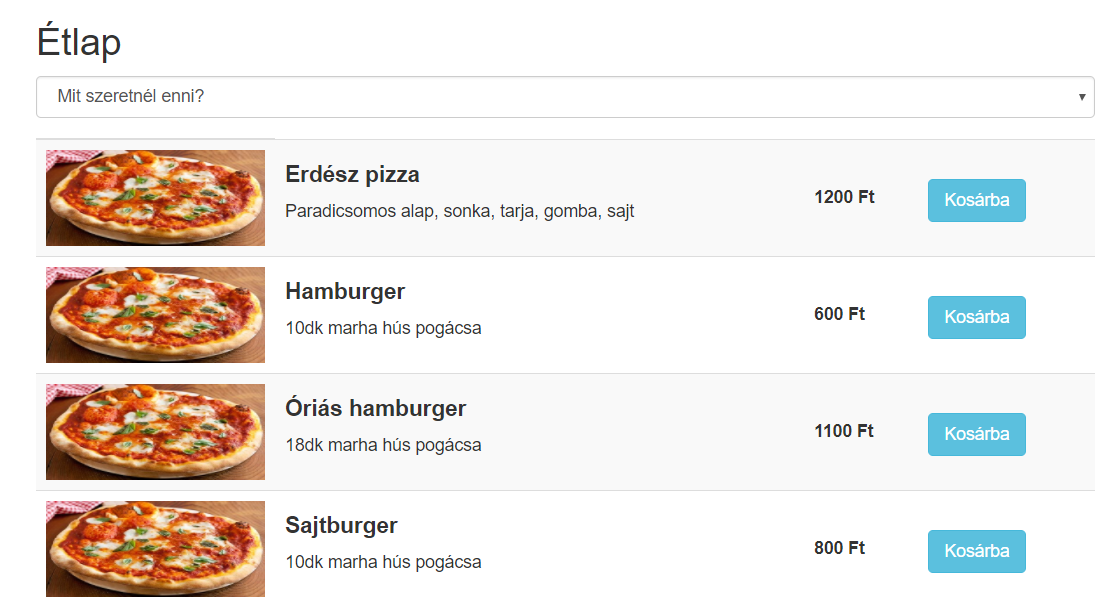
\includegraphics[scale=0.5]{kepek/menu.png}
\caption{Kép egy, az alkalmazásban megjelenített étlapról}
\label{fig:menu}
\end{figure}

\subsection{Fizetés}

A felhasználói felületen a kosár az étlap mellett, jobb oldalon található szintén egy táblázatos megoldással. A hozzáadott termékek neve és ára egymás alatt jelenik meg, egy végösszeggel a táblázat alján (\ref{fig:order}. ábra).

A kosár legalsó sorában egy „fizetés” gomb található. A gombra kattintva felugrik egy modal ablak, ahol egy legördülő menüből lehet kiválasztani a kívánt fizetési módot. Az alkalmazásban korlátozott számú fizetési lehetőség van, ami éttermenként változó lehet. Hogy egy étterem milyen fizetési lehetőségeket biztosít, azt az adott étterem felvitelekor kell megadni.

\begin{figure}
\centering
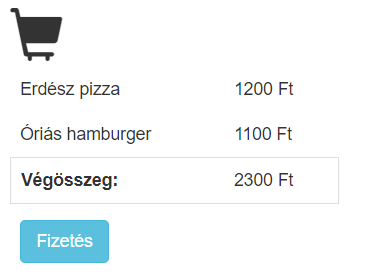
\includegraphics[scale=0.8]{kepek/order.png}
\caption{A vásárlás tételei összeggel és végösszeggel megjelenítve}
\label{fig:order}
\end{figure}

A kívánt fizetési lehetőség kiválasztása után (\ref{fig:payment}. ábra) a fizetés gombbal lehet véglegesíteni a megrendelést. Ilyenkor kapunk értesítést, hogy sikeres volt a rendelés.

\begin{figure}
\centering
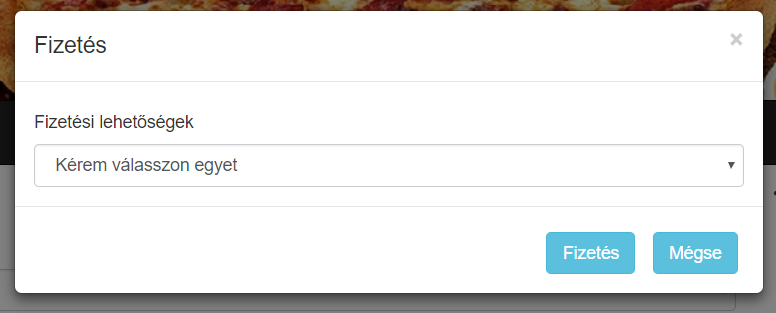
\includegraphics[scale=0.8]{kepek/payment.png}
\caption{A fizetési mód kiválasztása}
\label{fig:payment}
\end{figure}

\subsection{Profilom}

A profilom funkció kilistázza a bejelentkezett felhasználó adatait. Egy táblázatba foglalva kilistázza a felhasználó teljes nevét, felhasználónevét, email címét, telefonszámát, jutalompontját és címét/címeit. Egy felhasználónak akár több különböző szállítása címe is. A táblázat legalsó sorában van egy gomb „jelszó módosítása” felirattal (\ref{fig:profile}. ábra).

Jutalompontot a rendelések után kap a vásárló, minden elköltött 100 forint után egy jutalom pontot ír jóvá a rendszer. Az összegyűjtött pontokat, fizetéskor be lehet váltani, ilyenkor a beváltott pontok összege levonásra kerül a rendelés végösszegéből.

\begin{figure}
\centering
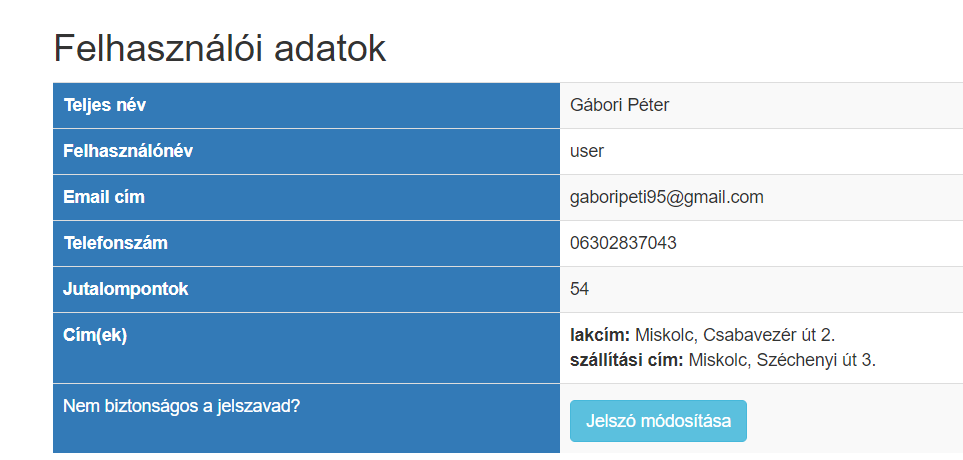
\includegraphics[scale=0.6]{kepek/profile.png}
\caption{Felhasználói adatok megjelenítése}
\label{fig:profile}
\end{figure}

A „Jelszó módosítása” gombra kattintva megjelenik egy űrlap, ahol a felhasználónak lehetősége van megváltoztatni a jelenlegi jelszavát (\ref{fig:password}. ábra). Meg kell adnia a jelenlegi jelszavát, majd az új jelszavát és végül meg kell erősítenie az új jelszót. Ha kitöltötte a bemeneti mezőket, a „Mentés” gombra kattintva megtörténik a jelszó cserélő funkció meghívása. Amennyibben a jelenlegi jelszó helyes, az új jelszó megfelel a kritériumoknak és megegyezik a megerősített jelszóval, megtörténik a jelszó módosítása.

\begin{figure}
\centering
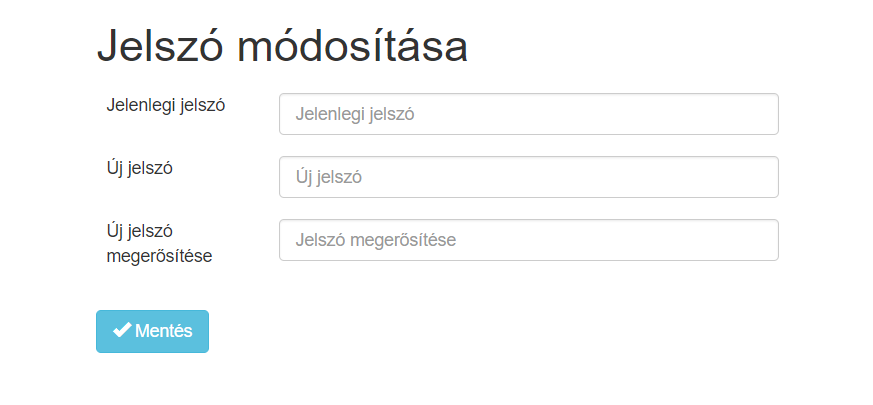
\includegraphics[scale=0.8]{kepek/password.png}
\caption{Jelszó megváltoztatása}
\label{fig:password}
\end{figure}

\section{Étterem tulajdonos funkciók}

\subsection{Éttermeim}

Az éttermeim funkció kilistázza a felhasználó adatbázisban szereplő éttermeit. Az éttermek táblázatos elrendezésben jelennek meg a felületen, a táblázat minden egyes sora, egy éttermet reprezentál. A táblázat oszlopaiban az éttermek különböző adatai találhatók, többek között az étterem logója, neve címe. A jobb szélső oszlopban három gomb található, „Étlap szerkesztése”, „Étterem szerkesztése” és a „Rendelések” (\ref{fig:my_restaurants}. ábra).

\begin{figure}
\centering
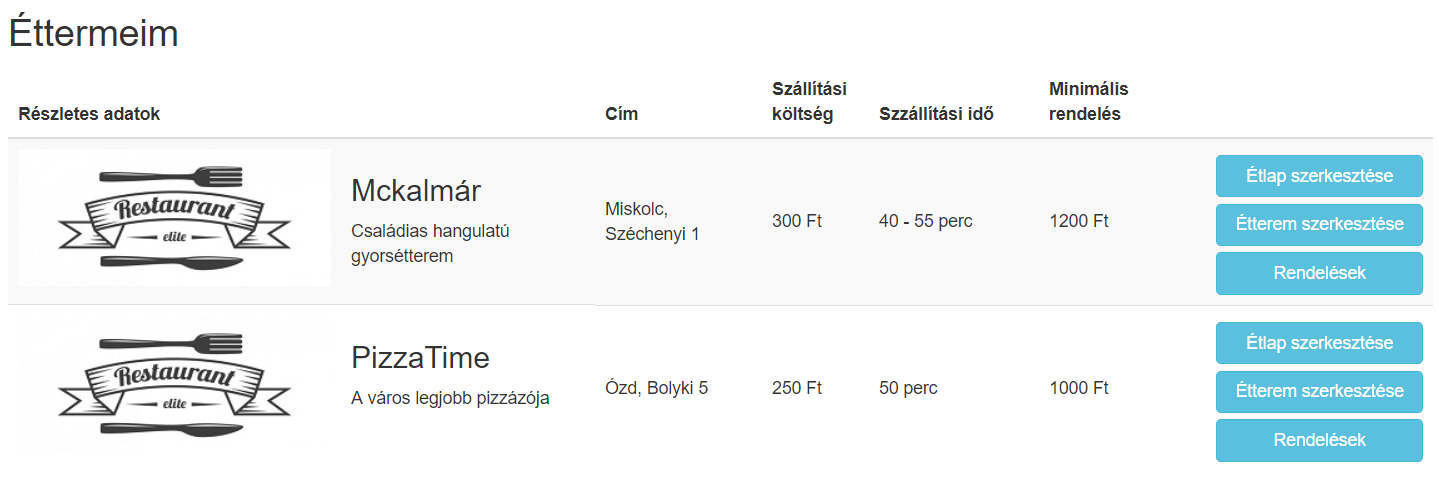
\includegraphics[scale=0.5]{kepek/my_restaurants.png}
\caption{A saját éttermek kilistázása}
\label{fig:my_restaurants}
\end{figure}

\subsection{Étlap szerkesztése}

Az étlap szerkesztése menüpont kiválasztása utána, egy táblázatot fogunk látni az adott étterem által forgalmazott ételekről és ezen ételek adatairól. Az elrendezés hasonló a user oldalon látott étlapok elrendezéséhez.

Az ételek egymás alatt, egy táblázatban jelennek meg. A táblázat egyes soraiban egy-egy étel szerepel, az oszlopaiban pedig az adott étel adatai. A táblázat jobb szélső oszlopában két gomb található, „Étel szerkesztése”, „Étel törlése”. A táblázat alatt egy „Étel felvitele” feliratú gomb van.

A táblázat felett egy legördülő menü van, amelynek segítségével a tulajdonos rá tud szűrni a különböző ételtípusokra, ezáltal könnyebben megtalálhatja a szerkeszteni, vagy törölni kívánt terméket. Az étel típus kiválasztása után, az ételek listája szűrve lesz az adott típus szerint, tehát csak a kívánt típusú ételek fognak megjelenni a táblázatban (\ref{fig:new_meal}. ábra).

\begin{figure}
\centering
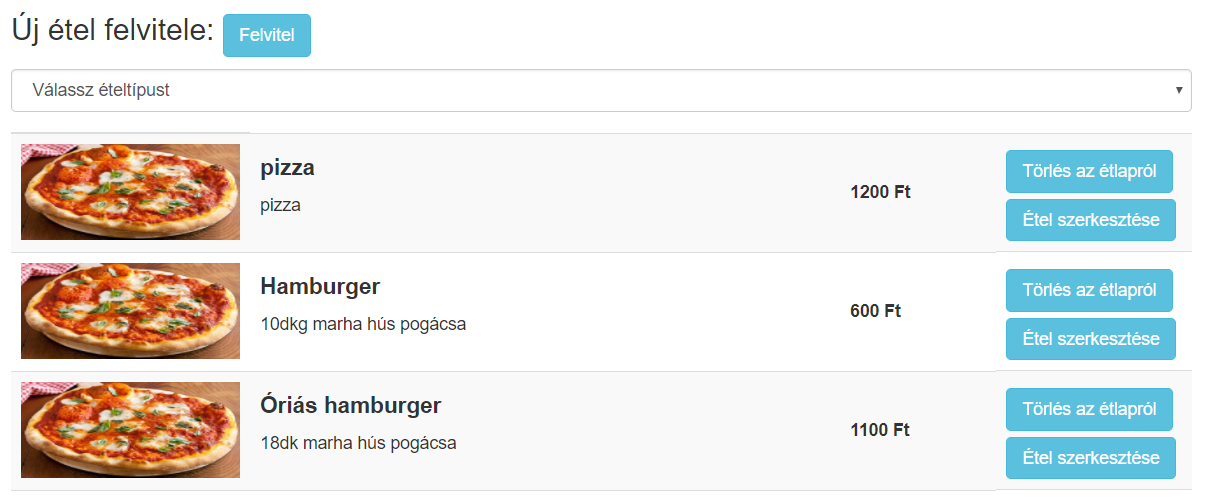
\includegraphics[scale=0.5]{kepek/new_meal.png}
\caption{Új étel hozzáadása}
\label{fig:new_meal}
\end{figure}

\subsection{Étel törlése}

Az étterem tulajdonosnak lehetősége van testre szabnia az étterme által biztosított kínáltaot. Vannak bizonyos ételek, melyeket csak szezonálisan lehet elkészíteni az alapszükségletük miatt, vagy csak valamilyen oknál fogva úgy dönt a vezetőség, hogy le kell kerülnie az étlapról. Ilyenkor van szükség az étel törlés funkcióra. Az „Étel törlése” gombra kattintva meghívásra kerül az étel törlése funkció, melynek hatására a kiválasztott étel törlődik a megjelenített ételek listájából, és törlődik az adatbázisból is.

\subsection{Étel szerkesztése}

Az étel szerkesztése funkcióval lehetőséget biztosítok az étterem tulajdonos számára, az étlapon szereplő termékek adatainak módosítására. Tehát ha egy adott ételnek megváltozik az ára vagy például az összetétele, akkor nem kell törölni azt, majd az új adatokkal ismét felvinni az adatbázisba. Mindössze rá kell kattintani a szerkeszteni kívánt termék sorában található gombok közül az „Étel szerkesztése” gombra, melynek hatására meghívódik az étel szerkesztése funkció.

Egy űrlapot fogunk látni, ahol a szükséges módosítások elvégzése után, a mentés gombbal lehet véglegesíteni a módosítást (\ref{fig:edit_meal}. ábra).

\begin{figure}
\centering
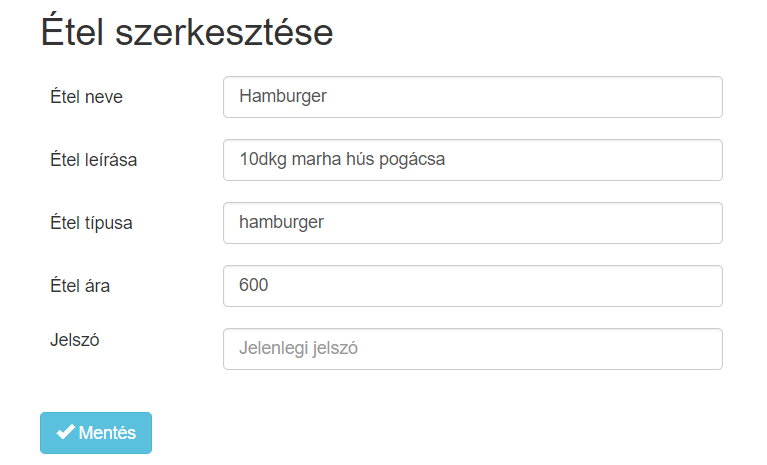
\includegraphics[scale=0.8]{kepek/edit_meal.png}
\caption{Egy étel adatainak szerkesztése}
\label{fig:edit_meal}
\end{figure}

\subsection{Étel felvitele}

Az étel felvitel gombra kattintva egy űrlap fog betöltődni. Az űrlap beviteli mezőkből áll, melyekkel az étlapra felvinni kívánt étel adatait tudjuk elküldeni a szervernek. Meg kell adni többek között az étel nevét, árát és típusát. Amennyiben minden szükséges mezőt kitöltöttünk a „Felvitel” gombra kattintva lehet véglegesíteni a műveletet.

\begin{figure}
\centering
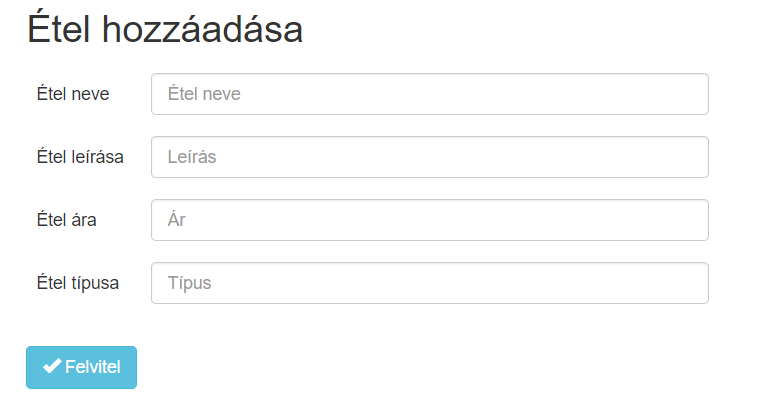
\includegraphics[scale=0.8]{kepek/add_meal.png}
\caption{Új étel felvitele az étlapra}
\label{fig:add_meal}
\end{figure}

\subsection{Rendelések}

Ahogy már említettem, az éttermeim funkció kilistázza a felhasználó adatbázisban szereplő éttermeit. Ilyenkor az éttermek táblázatos formában jelennek meg, minden étterem sorában szerepel egy „Rendelések” feliratú gomb. Erre a gombra kattintva a szerver kilistázza az adott étteremhez tartozó megrendeléseket, tehát azokat a rendeléseket, amiket ebben az étteremben adtak le a vásárlók. A rendelések táblázatos formában jelennek meg a felületen, egy sor egy rendelés. A táblázat oszlopaiban az egyes rendeléshez tartozó rendelési adatok vannak megjelenítve. Az adatok között szerepel a rendelő neve, rendelés időpontja, a megrendelt termékek, a rendelés összege és a fizetési módja.

\subsection{Étterem szerkesztése}

Egy étteremtulajdonosnak lehetősége lesz az éttermei adatainak módosítására. A szerkesztendő étterem sorában rá kell klikkelni az étterem szerkesztése gombra. Kattintás után megjelenik egy űrlap, amire fel kell vinni a módosítandó adatokat. Az adatok megadását követően a mentés gombbal lehet véglegesíteni a módosításokat (\ref{fig:edit_meal}. ábra).

\begin{figure}
\centering
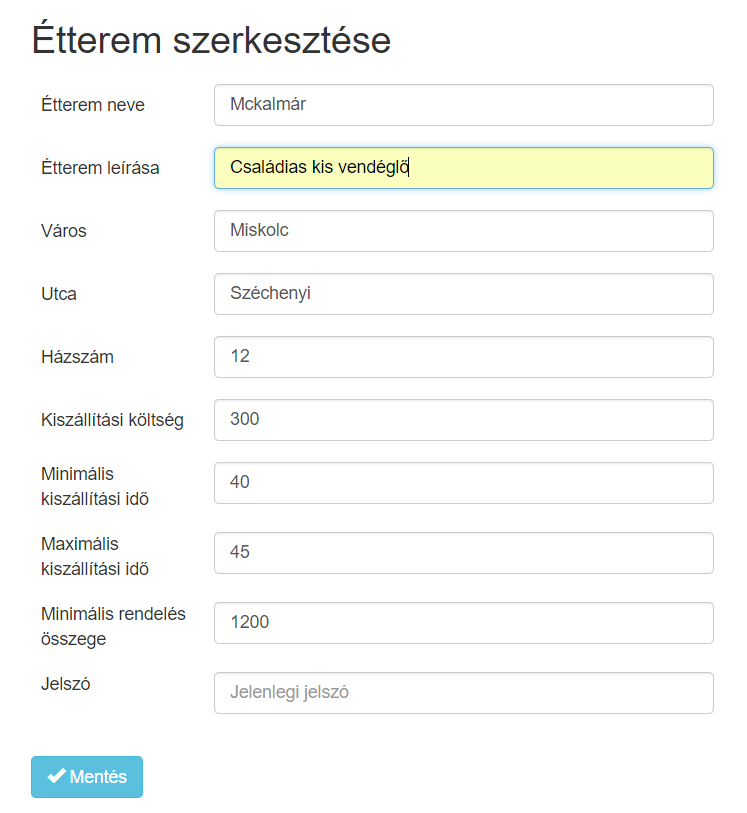
\includegraphics[scale=0.8]{kepek/edit_restaurant.png}
\caption{Étterem adatainak szerkesztése}
\label{fig:edit_restaurnt}
\end{figure}

\subsection{Étterem hozzáadása}

Egy étterem tulajdonosnak több étterme is lehet az adatbázisban. Az étterem hozzáadása menüpont alatt van lehetőség egy újabb éttermet felvinni. 
A menüpontra kattintva egy űrlapot fogunk látni, ahol a beviteli mezők egymás alatt helyezkednek el. Az egyes beviteli mezőkben az étterem különböző adatait lehet megadni. Az étterem nevét, leírását, címét. Ha elkészültünk az adatok megadásával, a „Felvitel” gombbal lehet véglegesíteni ezt a műveletet (\ref{fig:add_restaurant}. ábra).

\subsection{Profilom}

A profilom funkció az étterem tulajdonosok szempontjából is ugyanaz, mint a vásárlóknál. Kilistázza a bejelentkezett felhasználó adatait. Egy táblázatba foglalva kilistázza a felhasználó teljes nevét, felhasználónevét, email címét, telefonszámát és címét. A táblázat legalsó sorában van egy gomb „jelszó módosítása” felirattal.

A jelszó módosítás is ugyanúgy működik, mint a vásárlóknál. A „Jelszó módosítása” gombra kattintva megjelenik egy űrlap. Meg kell adni a jelenlegi jelszót, majd az új jelszót és végül meg kell erősíteni az új jelszót. A „Mentés” gombra kattintva megtörténik a jelszó cserélő funkció meghívása. Amennyibben a jelenlegi jelszó helyes, az új jelszó megfelel a kritériumoknak és megegyezik a megerősített jelszóval, megtörténik a jelszó módosítása.

\section{Felhasználói felület megvalósítása AngularJS segítségével}

A felhasználói felületet AngularJs segítségével valósítottam meg. Az app.js fájl tartalmazza az angular kódot. Az alkalmazásom egy single-page application, ami azt jelenti, hogy a weblap folyamatosan kis mennyiségű adatot cserél a szerverrel, tehát nem teljes HTML oldalak töltődnek le a szerverről, hanem egy adott oldal tartalma dinamikusan változik az alkalmazás használata során. A felhasználói felület különböző nézetekből épül fel. A nézetek HTML fájlokban tárolt HTML-kódrészletek. Egy nézet létrehozásához implementálni kell egy kontrollert és definiálni egy állapotot. A kontrollerek feladata a szerverrel való kommunikáció, és az adatok megjelenítése a nézeteken. A \texttt{\$stateProvider} modul kezeli az állapotokat, definiálásuk a .state() metódussal történik. Egy állapot definiálásakor meg kell adni a nevét, az URL-t amire aktiválódik, a HTML fájl elérési útját, amit be kell töltenie, tehát a nézetet, és azt, hogy melyik kontrollert használja. Az \texttt{\$urlRouterProvider} modul \texttt{.otherwise()} metódusa segítségével létrehoztam egy olyan állapotot, ami akkor aktiválódik, ha a hivatkozott URL egyik meglévő állapotra se illeszkedik. Ilyenkor egy hiba üzenetet tartalmazó nézet töltődik be.

Az angular fájlban definiálok egy \texttt{.run} blokkot is, amelyben a sütik értékeit frissítem, és biztosítom, hogy amíg a felhasználó nem jelentkezett be, csak a bejelentkező, és regisztráló felületet érhesse el.

A fejezet további részében az állapotokat és kontrollereket fogom részletezni.

\subsection{Állapotok}

Ahogy már korábban leírtam egy állapot definiálásakor meg kell adni a nevét, az URL-t amire aktiválódik, a HTML fájl elérési útját, amit be kell töltenie, tehát a nézetet, és azt, hogy melyik kontrollert használja. A következő képpel demonstrálom ezt:

\begin{cpp}
.state("/", {
    url: "",
    templateUrl: "/static/partials/home.html",
    controller: "loginController"
})
\end{cpp}

A fenti állapot a \texttt{/static/partials/home.html} nézetet tölti be a \texttt{loginController} segítségével, ami a bejelentkező felületet. A \texttt{loginController} a felhasználók be és ki jelentkezését, illetve az autentikációt valósítja meg. Az autentikáció megvalósításához létrehoztam egy \textit{service}-t, az \texttt{AuthenticationService}-t. Ezt a \texttt{service.js} fájl valósítja meg. Az hitelesítése folyamata során a kontroller meghívja az \texttt{AuthenticationService} login metódusát, és paraméterként átadja neki a felhasználó által megadott felhasználónevet és jelszót. A service a kapott adatokat elküldi a szervernek, és várja a választ. A szerver elvégzi a szükséges ellenőrzéseket, lekérdezéseket, token generálást, és választ küld a \textit{service}-nek. A \textit{service} a kapott választ továbbítja a kontroller felé. A kontroller megvizsgálja a választ, ha nem 200-as státuszkódot kap, akkor visszatér egy hibaüzenettel viszont, ha a 200-as státuszkódot kapott a hitelesítés sikeres volt, meghívja az \texttt{AuthenticationService} \texttt{SetCredentials} metódusát és át adja neki a felhasználó nevét, jelszavát és típusát, majd betölti a \texttt{/startpage} nézetet. A service \texttt{SetCredentials} függvénye egy \texttt{\$rootScope} változónak dictionary-ként értékül adja a kapott adatokat és a szerver által generált tokent, majd értékül adja a változót egy sütinek.

Kijelentkezés esetén a kontroller az \texttt{AuthenticationService} \texttt{ClearCredentials()} metódusát hívja meg, ami törli a bejelentkezéskor létrehozott sütit.

\bigskip

\noindent \texttt{/startpage}

A \texttt{/startpage} URL-re hivatkozva a \texttt{/static/partials/startpage.html} nézet töltődik be, ami a webalkalmazás nyitóoldala.

\bigskip

\noindent \texttt{/registration}

A \texttt{/registration} URL-re való hivatkozás a \texttt{/static/partials/registration.html} nézetet tölti be a userController segítségével. A kontroller betölti a regisztrációs felületet, a felhasználó felviszi az adatait, amiket a kontroller továbbít a szerver felé.

\bigskip

\noindent \texttt{/restaurant}

A \texttt{/restaurant} URL-re hivatkozva a \texttt{restaurantController} betölti a \texttt{/static/partials/restaurant.html} nézetet. A kontroller lekéri a szervertől az éttermeket. A megjelenített táblázatban biztosítja a városok szerinti szűrést.

\bigskip

\noindent \texttt{/myRestaurant}

A \texttt{myRestaurantController} a \texttt{/static/partials/my\_restaurants.html} nézetett tölti be a \texttt{/myRestaurant/:username} URL hivatkozás után. A kontroller lekéri a szervertől a paraméterként átadott azonosítóval rendelkező felhasználó éttermeit.

\bigskip

\noindent \texttt{/list-meals}

A \texttt{/list-meals/:restaurant\_id} URL-re hivatkozva a \texttt{mealsController} betölti a \texttt{/static/partials/list\_meals.html} nézetet. A kontroller lekéri a szervertől a paraméterként kapott étterem által kínált ételeket, az étterem által kínált ételek típusait és a fizetési módokat. A táblázatban megjelenített ételek között a kontroller szűrési lehetőséget biztosít a lekért típusok alapján. A kontroller létrehoz egy \texttt{\$rootScope} kosarat, amihez az \texttt{addToCart()} funkció meghívásával lehet ételeket hozzáadni. Az \texttt{addToCart()} kap egy ételt paraméterként, amit beletesz a kosár listába, majd a kosarat beleteszi egy sütibe. A \texttt{removeFromCart()} függvénnyel lehet a kosárból törölni, először a kosár listából törli a paraméterként kapott ételt, majd frissíti a süti tartalmát.

A kontrollerben definiálva van egy \texttt{checkout()} függvény, ami fizetéskor kerül meghívásra. Fizetés előtt ki kell választani a szervertől lekérdezett fizetési módok közül egyet. A fizetés-re kattintva meghívásra kerül a fentebb említett \texttt{checkout()} metódus, ami elküldi a szervernek a kosár tartalmát, a vásárló nevét, és a választott fizetési módot.

\bigskip

\noindent \texttt{/setting-meals}

A \texttt{/setting-meals/:restaurant\_id} URL-re hivatkozva a \texttt{mealsSettingController} betölti a \texttt{/static/partials/setting\_meals.html} nézetet. A kontroller lekéri a szervertől a paraméterként megadott étterem ételkínálatát, és az étterem által forgalmazott ételek típusait. A lekérdezett ételeket egy táblázatban jeleníti meg, ahol ételtípus szerinti szűrési lehetőséget is biztosít.

A kontrollerben definiálva van egy \texttt{removeMeal()} függvény, ami a paraméterként kapott étel objektumot elküldi a szervernek, a szerver törli az adatbázisból, majd visszatér egy státuszkóddal.

\bigskip

\noindent \texttt{/add-meal}

Az \texttt{/add-meal} állapot a \texttt{/add-meal/:restaurant\_id} URL-re hivatkozva érhető el. A hivatkozás során a \texttt{mealsAddController} betölti a \texttt{/static/partials/add\_meal.html} nézetet. A kontrollernek egyetlen \texttt{addMeal()} metódusa van, ami az új étel felviteléért felelős. A metódus kap egy étel objektumot, ami a felhasználó által megadott adatokat tartalmazza. A szervernek paraméterként elküldi a kapott objektumot, és a módosítandó étterem azonosítóját. A szerver elvégzi a szükséges adatbázismódosításokat, majd visszatér egy státuszkóddal.

\bigskip

\noindent \texttt{/addRestaurant}

Az \texttt{/addRestaurant} URL-en a \texttt{/static/partials/add\_restaurant.html} nézet érhető el, melynek megjelenítéséért az \texttt{addRestaurantController} a felelős. A kontrollerben van egy \texttt{addRestaurant()} függvény, amit meghívva elküldi a szervernek a paraméterként kapott adatokat, és a bejelentkezett felhasználó nevét. A szerver elvégzi a módosításokat, felviszi az adatbázisba az új éttermet, majd sikeres adatbázisműveletek esetén 200-as státuszkódot küld vissza válaszként.

\bigskip

\noindent \texttt{/my-orders}

A \texttt{/static/partials/get\_orders.html} nézet a \texttt{/my-orders/:restaurant\_id} URL-en érhető el. A nézet megjelenítését az \texttt{ordersController} végzi. A kontroller lekéri a szervertől a paraméterként kapott étteremben leadott összes rendelést, majd egy táblázatban megjeleníti azokat.

\bigskip

\noindent \texttt{/my-profile}

A \texttt{/my-profile} URL-re hivatkozva elérhetjük a \texttt{/static/partials/my\_profile.html} nézetet, melyet a \texttt{userProfileController} jelenít meg. A kontroller lekéri a szervertől az aktuális bejelentkezve lévő felhasználó felhasználói adatait.

\bigskip

\noindent \texttt{/edit-profile}

Az \texttt{/edit-profile/:user\_id} URL-re való hivatkozás után a \texttt{userSettingsController} megjeleníti a \texttt{/static/partials/edit\_password.html} nézetet. A kontroller lekéri a szervertől az aktuális bejelentkezve lévő felhasználó felhasználói adatait. A kontrollerben definiálva van egy \texttt{editUser()} metódus, ami paraméterként elküldi a szervernek a lekért felhasználói adatokat, és a felhasználói felületről kapott adatokat. A szerver feldolgozza az adatokat, elvégzi az ellenőrzéseket, és módosítja a felhasználó jelszavát. Sikeres módosítás esetén 200-as státuszkódot küld vissza válaszként.

\bigskip

\noindent \texttt{/edit-restaurant}

Az \texttt{editRestaurantController} betölti a \texttt{/static/partials/edit\_restaurant.html} nézetet az \texttt{/edit-restaurant/:restaurant\_id} URL-re hivatkozás után. A kontroller lekéri a szervertől a paraméterként kapott étterem adatait. A kontrollerben definiált \texttt{editRestaurant()} függvény paraméterként elküldi a szervernek a lekérdezett étterem adatait, és a felhasználói felületről kapott módosítandó adatokat. A szerver elvégzi a szükséges ellenőrzéseket és adatbázismódosításokat, majd visszatér egy státuszkóddal.

\bigskip

\noindent \texttt{/edit-meal}

A \texttt{/static/partials/edit\_meal.html} nézetet a \texttt{/edit-meal/:meal\_id} URL-en lehet elérni. A nézetet az \texttt{editMealController} jeleníti meg. A kontroller lekéri a szervertől a paraméterként kapott étel adatait. A kontrollerben definiált \texttt{editMeal()} metódus paraméterként elküldi a szervernek a lekérdezett étel adatait, az ételt forgalmazó étterem azonosítóját, és a felhasználói felületről kapott módosítandó adatokat. A szerver elvégzi a szükséges ellenőrzéseket és adatbázismódosításokat, majd visszatér egy státuszkóddal.

% \chapter{Alapfunkciók bemutatása}

Ez nem feltétlen jó így fejezet címnek, pontosabban ezen a témán belül több fejezet is lehet, attól függően, hogy majd mivel és hogy sikerül elkészülni.

Itt kb. olyasmire kell gondolni, mint
- rendelések nyilvántartása,
- promóciók, törzsvásárlói kedvezmények megvalósítása a rendszerben,
- nyersanyagok nyilvántartása,
- rendelési statisztikák, elemzés, megjelenítés,
- ...

Annyi biztos, hogy a címnek megfelelően a rendeléseket majd nyilván kell tartani. A többi ahhoz kapcsolható funkció, de csak akkor célszerű vele foglalkozni, ha az alapfunkciók már megvannak.

A tervezéséről szóló dolgokat az alkalmazás felépítésénél is el lehet kezdeni, de ott még inkább csak az interfészekre, az API jellegére, konvenciókra, illesztési módokra vonatkozóan.

Magában az implementációba annyira kell csak majd belemenni az alapfunkciók bemutatásánál, hogy a kiemelt kódpéldák alapján át lehessen tekinteni a rendszer egészét, és a leírás alapján aki akarja hellyel-közzel tuda is reprodukálni a rendszert.

\section{Statisztikai jellegű elemzések}

Felhasználói szokások elemzése

Rendelések száma (idő függvényében)
Rendelések összege
Fizetési módok gyakorisága
Ételek típusai
Felhasználók rendelésszámának eloszlása
Nap melyik szakában történt a rendelés (ehhez is eloszlás)

Felhasználók osztályozása/klaszterezése
- osztályozásnál eleve tudjuk, hogy mi a csoport jellemzője.
- klaszterezésnél adottak a mintáink, szeretnénk megtudni, hogy milyen csoportok vannak benne.

\section{Ajánlórendszer}

Piaci kosár elemzés

Amit meg kellene nézni:
- Milyen termékhez milyen másik terméket érdemes ajánlani?
- Mikor célszerű az akciókat meghírdetni és milyen termékekre vonatkozóan? (Például hónap elején-végén, karácsonykor, szezonalitást vizsgálni)
- Felhasználónként mikor lehet külön üzenetet küldeni egy-egy akcióról? (Észrevétel: Nem érdemes túl sok akciót küldeni gyakran, mert spam lesz belőle.)

\Chapter{Tesztelés}

Miden szoftverben van hiba. A szoftvereket emberek fejlesztik, és az emberek hibáznak, ezért van szükség a programok tesztelésére. A szoftver termékben lévő hibák nagy részét még a végleges üzembe helyezés előtt ki lehet szűrni a tesztek segítségével. A tesztelések segítségével növelhetjük a program megbízhatóságát, minőségét. Teszteléssel se lehet minden hibát kiszűrni, ugyanis nagyobb rendszereknél nem lehetséges minden bemenetet tesztelni. Érdemes a teszteléseket a szoftver életciklusának korai szakaszában elkezdeni, mert minél hamarabb találjuk meg a hibát annál költséghatékonyabb a javítása.

Több fajta tesztelési technikát különböztetünk meg. Beszélhetünk specifikáció alapú tesztről, amikor a tesztelő számára nem áll rendelkezésre a forráskód, és a specifikáció alapján készülnek a tesztek. Illetve létezik strukturális tesztelés, amikor egy kész struktúrát tesztelünk, például osztályokat, funkciókat vagy metódusokat.

\Section{Tesztelés szintjei}

A tesztelésnek több szintje is van, léteznek teljes rendszer tesztek,	 amikor azt ellenőrzik, hogy a termék megfelel-e a specifikációnak. A rendszerteszt már a kész terméket ellenőrzi. A rendszerteszteket gyakran független cég végzi. Fontos, hogy a tesztkörnyezet minél inkább hasonlítson a megrendelő környezetére.

A tesztelés egy másik szintje az integrációs teszt. Az integrációs teszt az elkészült modulok együttes működését teszteli. Tesztelik a komponensek közti interfészeket, illetve a más rendszerek felé nyújtott interfészeket is.

A tesztelések legalsó a szintje a komponensteszt. A komponensteszt külön-külön teszteli a rendszer egyes komponenseit. Két gyakran használt fajtája van a komponensteszteknek, a modulteszt és a unit-teszt. A modulteszttel általában a nem-funkcionális részeket szokták tesztelni, például azt, hogy van e memory leak.

\Section{Unit-test}

Az egységteszt a funkciókat teszteli. Ismerjük a metódus visszatérési értékét egy adott bemeneti paraméterre, ha a tényleges visszatérési érték egyezik az elvárt értékkel, akkor a teszt sikeres, különben sikertelen. A unit-tesztek lényege, hogy a szoftverben történt változtatás után csak újra le kell futtatni a meglévő egységteszteket, és ha egyik teszt eset se bukik el, akkor a változtatás nem okozott hibát a rendszerben.
A unit-tesztek egyik nagy előnye, hogy a legtöbb fejlesztő környezet támogatja őket, tehát egyszerű az implementálásuk. A Phyton esetén is van egy egységtesztelő keretrendszer, amire PyUnit néven szoktak hivatkozni.

A PyUnit a JUnit Python nyelvű változata \cite{python_test}. Támogatja a tesztek automatizálását, összegyűjtésüket gyűjteménybe, és a tesztek függetlenségét. Az alkalmazásom szerveroldalának tesztelésére unit-teszteket használtam.

\begin{python}
from tests.base import BaseTestCase
from nyilvantarto.user import query_users

class UserEmptyTestCase(BaseTestCase):
 """Test cases for testing the user class"""
    def test_no_users(self):
        person_results = query_users()
        self.assertEqual(person_results, [])

    def test_add_user(self):
        user_registration(newUser=
            {'user_name': 'user_name', 'password': 'name',
             'first_name': 'first', 'last_name': 'last',
             'phone_number': '06202587854', 'email': 'email',
             'city': 'miskolc', 'street': 'f\"o',
             'number': '1'})

        person_results = query_users()
        self.assertEquals(len(person_results), 1)
        result = person_results[0]
        self.assertEquals(result['user_name'], 'user_name')
\end{python}

\newpage

Fentebb látható két teszt példa. Az elsővel azt tesztelem, hogy ha egy üres adatbázisra meghívom a felhasználók lekérdezéséhez szükséges függvényt, akkor egy üres listát ad-e vissza. A teszt sikeresen lefutott. A második tesztben egy új felhasználót viszek fel az adatbázisra, és utána ismét lekérdezem az adatbázisban lévő felhasználókat. Lekérdezés után vizsgálom, hogy egy darab felhasználó van-e a lekérdezés eredményében, illetve, hogy egyezik-e a neve a felvitt felhasználó nevével. Ez a teszt is sikeresen lefutott.

\Section{Front-end tesztelése}

Az alkalmazásom front-end oldalát AngularJS segítségével valósítom meg \cite{angular_test}. Az AngularJS-be számos olyan funkciót, eszközt építettek, amik megkönnyítik a kódok tesztelését. Az Angular kódok a teszteléséhez ezeket az eszközöket kell használni. Ilyen eszköz például a Jasmine.

A Jasmine egy viselkedésvezérelt fejlesztési keretrendszer a JavaScript alapú nyelvek számára. A Jasmine a legnépszerűbb keretrendszer, melyet AngularJS kódok tesztelésére használnak. A Jasmine olyan funkciókat biztosít, melyek segítenek a tesztek struktúrájának kialakításában. Ahogy a tesztek növekednek, egyre fontosabb a jól strukturáltság fenntartása, a Jasmine segít elérni ezt.

\chapter{Összegzés}

A szakdolgozatom célja egy olyan webalkalmazás készítése volt, amellyel éttermek és rendelések adatait lehet nyilvántartani. Célom volt a felhasználók számára egy egyszerű, letisztult, felhasználóbarát felület kialakítása, amelyen szűrési lehetőségek segítségével könnyen el lehet navigálni az éttermek kínálatai között. Továbbá kitűzött cél volt az étteremtulajdonosok munkájának megkönnyítése, az éttermek menedzselésének a leegyszerűsítése. Az adatokat SQL alapú relációs adatbázisban tárolom, amelyhez a keretrendszer SQLAlchemy ORM-en keresztül csatlakozik. Az alkalmazásom megvalósításához szerveroldalon Python/Flask keretrendszert használtam, míg a kliensoldali megvalósítás AngularJS segítségével történt.

Az alkalmazás a jelenlegi állapotában működőképes, a tervezett funkcionalitásokat sikeresen implementáltam. Van néhány ötletem az alkalmazás későbbi továbbfejlesztéséhez. Az egyik, ötletem az ajánlórendszer megvalósítása, aminek a részletei a dolgozat második fejezetében már részletesen kifejtésre került. Egy másik ötletem, egy nyersanyag nyilvántartó rendszer bevezetése. Az étterem tulajdonosoknak lehetőségük lenne az ételek készítéséhez használt nyersanyag készletük nagyságát felvinni az adatbázisba. Amikor valamelyik nyersanyag készleten lévő darabszáma egy előre meghatározott kritikus érték alá csökken, a rendszer figyelmeztető üzenetet küldene a tulajdonos számára. Hasznos lenne még a rendelési statisztikák és elemzések bővítése is.


\Chapter{CD-melléklet tartalma}

A szakdolgozatom mellé egy darab CD tartozik, amely a következő adatokat tartalmazza.

\bigskip

\noindent \texttt{Dolgozat} katalógus:

\begin{itemize}
\item \texttt{feladat\_kiiras.pdf}: A feladatkiírást tartalmazó fájl, PDF formátum.
\item \texttt{összefoglalás.pdf}: A dolgozat magyar nyelvű összefoglalása, PDF formátumban.
\item \texttt{összefoglalás.tex}: A dolgozat magyar nyelvű összefoglalása, \LaTeX formátumban.
\item \texttt{summary.pdf}: A dolgozat angol nyelvű összefoglalása, PDF formátumban.
\item \texttt{summary.tex}: A dolgozat angol nyelvű összefoglalása, \LaTeX formátumban.
\end{itemize}

\bigskip

\noindent LaTeX katalógus:

A dolgozatom \LaTeX kódját tartalmazza.

\bigskip

\noindent \texttt{Éttermi rendelés-nyilvántartó\_rendszer.pdf}:

A dolgozatomat tartalmazó PDFfájl.

\bigskip

\noindent \texttt{Forraskód} katalógus:

Az alkalmazásom forráskódját tartalmazza.


\begin{thebibliography}{x}
\addcontentsline{toc}{chapter}{\bibname}

\bibitem{python}
Python, \url{https://www.python.org/about}

\bibitem{flask}
Flask, \url{http://flask.pocoo.org/docs/0.12}

\bibitem{sqlalchemy}
SQLAlchemy, \url{https://www.sqlalchemy.org}

\bibitem{html}
HTML, \url{https://www.w3.org/TR/html52}

\bibitem{javascript}
JavaScript, \url{https://developer.mozilla.org/hu/docs/Web/JavaScript}

\bibitem{angularjs}
AngularJS, \url{https://docs.angularjs.org/guide}

\bibitem{css}
CSS, \url{https://www.w3.org/Style/CSS/Overview.en.html}

\bibitem{bootstrap}
Bootstrap, \url{https://getbootstrap.com/docs/3.3}

\bibitem{git}
Git, \url{https://git-scm.com/about}

\bibitem{github}
GitHub, \url{https://github.com/features}

\bibitem{sqlite}
GitHub, \url{https://www.sqlite.org/docs.html}

\bibitem{pycharm}
GitHub, \url{https://www.jetbrains.com/help/pycharm/2017.1/general-guidelines.html?utm_medium=help_link&utm_source=from_product&utm_campaign=PY&utm_content=2017.1}


\bibitem{pizza.hu}
GitHub, \url{https://www.pizza.hu/}

\bibitem{falatozz.hu}
GitHub, \url{https://falatozz.hu/}

\bibitem{netpincer.hu}
GitHub, \url{https://www.netpincer.hu/}

\bibitem{foreign_restaurant_sofwares}
GitHub, \url{https://www.capterra.com/restaurant-management-software/}

\bibitem{jwt}
GitHub, \url{https://jwt.io/introduction/}

\bibitem{canvasj}
GitHub, \url{https://canvasjs.com/}

\bibitem{owl}
GitHub, \url{http://pagesperso.lina.univ-nantes.fr/~skaf-h/pmwiki/uploads/Main/owlSytaxManchester.pdf}

\bibitem{recommender_system}
GitHub, \url{http://www.inf.u-szeged.hu/~ormandi/presentations/recommenderSystem.pdf}

\bibitem{compare_restaurant_softwares}
GitHub, \url{http://vendeglatoprogram.blogspot.hu/}

\bibitem{compare_restaurant_softwares}
GitHub, \url{http://vendeglatoprogram.blogspot.hu/}

\bibitem{esystem}
GitHub, \url{http://vendeglatoprogram.com/ettermi-szoftver}

\bibitem{standmagus}
GitHub, \url{http://www.vendeglato-szoftver.hu/}

\bibitem{compassz}
GitHub, \url{http://www.com-passz.hu/}


\end{thebibliography}


\pagestyle{empty}
\vspace*{1cm}  
\begin{center}
\large\textsc{\bfseries Eredetiségi Nyilatkozat}
\end{center}
\vspace*{2cm}  

Alulírott \textbf{Gábori Péter Márk}; Neptun-kód: \texttt{TECWTE} a Miskolci Egyetem Gépészmérnöki és Informatikai Karának végzõs mérnökinformatikus szakos hallgatója ezennel büntetõjogi és fegyelmi felelõsségem tudatában nyilatkozom és aláírásommal igazolom, hogy
\textit{Éttermi rendelésnyilvántartó rendszer}
címû szakdolgozatom/diplomatervem saját, önálló munkám; az abban hivatkozott szakirodalom
felhasználása a forráskezelés szabályai szerint történt.\\

Tudomásul veszem, hogy szakdolgozat esetén plágiumnak számít:
\begin{itemize}
\item szószerinti idézet közlése idézõjel és hivatkozás megjelölése nélkül;
\item tartalmi idézet hivatkozás megjelölése nélkül;
\item más publikált gondolatainak saját gondolatként való feltüntetése.
\end{itemize}

Alulírott kijelentem, hogy a plágium fogalmát megismertem, és tudomásul veszem, hogy
plágium esetén szakdolgozatom visszautasításra kerül.

\vspace*{3cm}

\noindent Miskolc, \hbox to 2cm{\dotfill} év \hbox to 2cm{\dotfill} hó \hbox to 2cm{\dotfill} nap

\vspace*{3cm}

\hspace*{8cm}\begin{tabular}{c}
\hbox to 6cm{\dotfill}\\
Hallgató
\end{tabular}


\end{document}
